\input preamble.tex

\begin{document}
\linenumbers

\title[MAC6962 Tópicos Matemáticos para Computação Contemporânea]{%
{\small\sl Sinopse das aulas}\\\bigskip
MAC6962 Tópicos Matemáticos para Computação Contemporânea\\\bigskip
{\it Segundo Semestre de 2019}
}

\address{Instituto de Matemática e Estatística, Universidade de São
  Paulo, Rua do Matão 1010, 05508--090~São Paulo, SP}

% \email{}
%\thanks{}
%\begin{abstract}
%\end{abstract}

\yyyymmdddate
\shortdate
\def\today{\number\year/\number\month/\number\day}
\settimeformat{ampmtime}
\date{\today, \currenttime}
\footskip=28pt

%\keywords{}
%\subjclass[2010]{}

\maketitle

\section*{}
\label{sec:prefacio}
\doublespace
Notas de aula produzidas por
\begin{enumerate}[label=\nplain]
  \item Gabriel Morete de Azevedo,
  \item \dots João Pedro Turri,
  \item \dots,
  \item \dots\ e
  \item Vitor Santa Rosa Gomes.
\end{enumerate}

\endgroup
\newpage\onehalfspace
\tableofcontents
\pagestyle{fancy}

\endgroup
\doublespace
%\onehalfspace

\newpage
\part{CONCENTRAÇÃO DE MEDIDA}

\section{...}
\label{...}

\section{Aula 05 de Agosto de 2019}
\label{2019_08_05}

\subsection{Filtros de Bloom}

Considere o seguinte problema: dado um $S \subseteq \mathcal{U}$ e $x
\in \mathcal{U}$, decidir se $x \in S$. A solução para esse problema
consiste em montar alguma Estrutura de Dados para representar $S$,
como por exemplo uma tabela de hash ou uma árvore binária de busca
(ABB), e fazer consultas nessa estrutura. Queremos que a nossa solução
seja eficiente em tempo e espaço, sendo que o tempo consiste no tempo
de montar a estrutura (pré-processamento) e no tempo de resposta para
cada $x$ (consulta).

Na Tabela \ref{tab:tempo_problema_pertinencia}, temos o tempo de
pré-processamento e consulta utilizando hashing e ABB. Observe que nas
duas soluções a quantidade de espaço utilizado é $O(n)$. Queremos
gastar menos memória, para isso vamos permitir aleatorização e falsos
positivos.

\begin{table}[h]
\begin{tabular}{l|c|c|}
\cline{2-3}
                                       & \multicolumn{2}{c|}{\textbf{Tempo}}                                                      \\ \cline{2-3} 
                                       & \multicolumn{1}{l|}{\textbf{Pré-processamento}} & \multicolumn{1}{l|}{\textbf{Consulta}} \\ \hline
\multicolumn{1}{|l|}{\textbf{Hashing}} & $O(n)$                                          & $O(1)$                                 \\ \hline
\multicolumn{1}{|l|}{\textbf{ABB}}     & $O(n\lg n)$                                    & $O(\lg n)$                            \\ \hline
\end{tabular}
  \caption{Tempo utilizando Hashing e ABB}
  \label{tab:tempo_problema_pertinencia}
\end{table}

Mais precisamente, teremos:

\begin{enumerate}
\item Se $x \in S$, $\mathbb{P}(A(x)=1)=1$
\item Se $x \notin S$, $\mathbb{P}(A(x)=1) \leq \delta$.
\end{enumerate}

onde $A(x)$ é a solução desejada com $x$ como entrada.

\subsubsection{Primeira Tentativa}
  
Suponha que temos uma função de hashing
$h: \mathcal{U} \rightarrow T$, onde $|T|=m$. Vamos considerar que $h$
tem a seguinte propriedade: $h(u)$, para todo $u \in \mathcal{U}$, são
uniformemente distribuído em $T$ $\left(
\mathbb{P}(h(u)=t)=\frac{1}{m}\right)$ e são mutuamente independentes (essa
propriedade é usual em análises).

Vamos representar o conjunto $S$ utilizando um vetor $v$ de $m$
bits. Isto é:

\begin{align*}
v = (v_{t})_{t \in T} = (v(t))_{t\in T} \in \{0,1\}^{m}
\end{align*}

com

\begin{align*}
  v_{t}=\begin{cases}
    1, \text{ se } \exists s \in S : h(s)=t \\
    0, \text{ c/c. }
 \end{cases}
\end{align*}

Neste caso, o algoritmo $A$ devolverá $1$ se $v(h(x))=1$ e $0$ caso
contrário. Logo, $A(x)=v(h(x))$. Observe que se $x \in S$, então
$A(x)=1$ com probabilidade $1$ e se $x \notin S$, então
$\mathbb{P}(A(x)=1)\leq \frac{|S|}{|T|}$.

Consequentemente, para termos a probabilidade de falsos positivos
menor que $\delta$, basta tomarmos $|T| \geq
\frac{|S|}{\delta}$. Portanto, gastamos $\frac{1}{\delta}$ bits por
elemento de $S$. Queremos diminuir $\frac{1}{\delta}$ para
$O(\lg \frac{1}{\delta})$.

\subsubsection{Filtros de Bloom}

Neste caso, usamos $k$ funções de hashing
$h_{1},\dots,h_{k}:\mathcal{U} \rightarrow T$ e vamos assumir que
$h_{i}(u) (1 \leq i \leq k, u \in \mathcal{U})$ são uniformemente
distribuídas em $T$ e são mutuamente independentes. Como na tentativa
anterior, ainda vamos representar $S$ utilizando um vetor $v$ de $m$
bits, mas dessa vez:

\begin{align*}
  v_{t}=\begin{cases}
    1, \text{ se } \exists i \text{ e } s \in S : h_{i}(s)=t \\
    0, \text{ c/c. }
  \end{cases}
\end{align*}

Ademais:

\begin{align*}
  A(x)=\begin{cases}
    1, \text{ se } \forall i v(h_{i}(x))=1\\
    0, \text{c/c.}
  \end{cases}
\end{align*}

Claramente, se $x \in S$, então $A(x)=1$ com probabilidade 1. Queremos
estimar $\mathbb{P}(A(x)=1)$ para $x \notin S$. Lembre que $n=|S|$ e
$m=|T|$. Tomamos $m=n\frac{\lg_{2} 1/\eps}{\log 2}$ e $k=(\log 2)\frac{m}{n}$,
onde vamos escolher $\eps$ mais a frente \footnote{quando não crucial,
omitimos $\lfloor . \rfloor$ e $\lceil . \rceil$. Além disso,
$\lg=\lg_{e}=\log$}.

Como é $v=(v_{t})$? Temos:

\begin{align}
\mathbb{P}(v_{t}=0) &= \left(1-\frac{1}{m}\right)^{kn}\\
                    &= \left(e^{-\frac{1}{m}+O\left(\frac{1}{m^2}\right)}\right)^{kn} \label{eq:pr_vt_0}, & \left(\text{usando que } 1+x=e^{x+O(\frac{1}{x^2})}\right) \\
                    &= \frac{1}{2}e^{O\left(\frac{1}{m}\right)} \geq \frac{m}{2}\left(1-\frac{e}{2}\right), & (m \geq m_{0}(\eps))
\end{align}

Observe que em \eqref{eq:pr_vt_0}, assumimos que $O$ não tem
sinal. Iremos assumir isso no restante das aulas. Agora, seja $M_{0}$
uma variável aleatória tal que $M_{0}=\#0s$ em $v$. Então:

$$
\mathbb{E}(M_{0})=m\mathbb{P}(v_{t}=0) \geq \frac{m}{2}\left(1-\frac{\eps}{2}\right)
$$

\begin{fato}
\label{fato:filtros_de_Bloom}
$\mathbb{P}(M_{0} \leq \frac{m}{2}(1-\eps)) \leq e^{-c_{\eps}m}$, onde $c_{\eps} > 0$ depende apenas de $\eps$.
\end{fato}

Dado o fato acima, supomos que $M_{0} \geq \frac{m}{2}(1-\eps)$. Logo,
$M_{1}=m-M_{0} \leq \frac{m}{2}(1+\eps)$. Assim, se $x \notin S$, então:

\begin{align*}
  \mathbb{P}(A(x)=1)&= \left(\frac{M_{1}}{m}\right)^k \\
                    &\leq \left(\frac{1}{2}(1+\eps)\right)^k \\
                    &= \eps(1+\eps)^{\lg_{2}1/\eps}, & \left(k=\lg_{2}1/\eps\right)\\
                    &\leq \eps e^{\eps\lg_{2}1/\eps}, & \left(\text{usando que } (1+x) \leq e^{x}\right)\\
                    &= \eps e^{\lg\eps^{-\eps}/\lg 2}\\
                    &= \eps \eps^{-\eps/\lg 2}\\
                    &\leq 2 \eps, & \left(\text{para algum } 0 \leq \eps_{0} \leq \eps\right)\\
                    &= \delta
\end{align*}

tomando $\eps=\frac{\delta}{2}$. Portanto,
$m=n\frac{\lg 2/\delta}{\lg 2}$, ou seja, gastamos
$O(\lg \frac{1}{\delta})$ para cada elemento de $S$.

Agora vamos provar o Fato \ref{fato:filtros_de_Bloom}. Para isso,
vamos usar um resultado de concentração de variáveis aleatórias
conhecida como a desigualdade de McDiamird ou o método das diferenças
limitadas:

\begin{lema}[McDiamird \cite{mcdiarmid_method_89}]
\label{lema:McDiamird}
Suponha que $X_{1},\dots,X_{n}$ são variáveis aleatórias
independentes, com $X_{i}$ tomando valores em um conjunto $A_{i}(1
\leq i \leq n)$. Suponha que $f: A_{1}\times \dots A_{n} \rightarrow
\RR$ é tal que $|f(x)-f(x')|\leq c_{i}$ para quaisquer $x$ e $x' \in
A_{1}\times \dots \times A_{n}$ que diferem apenas na $i$-ésima
coordenada. Considere a variável aleatória
$Y=f(X_{1},\dots,X_{n})$.Para todo $t > 0$:

  \begin{enumerate}
    \item $\mathbb{P}(Y \geq \mathbb{E}(Y_0)+t) \leq e^{\frac{-2t^{2}}{\sum c_{i}^{2}}}$
    \item $\mathbb{P}(Y \geq \mathbb{E}(Y_0)-t) \leq e^{\frac{-2t^{2}}{\sum c_{i}^{2}}}$
    \end{enumerate}
\end{lema}

Portanto:

\begin{proof}[Demonstração do Fato \ref{fato:filtros_de_Bloom}]
Tomando $t = \frac{\eps m}{4}$, temos:

\begin{align*}
  \mathbb{E}(M_{0}) - t &\geq \frac{m}{2}\left(1-\frac{\eps}{2}\right) - t\\
                        &= \frac{m}{2}\left(1-\frac{\eps}{2}\right) - \frac{\eps m}{4}\\
                        &= \frac{m}{2}\left(1-\eps\right)
\end{align*}

Logo, usando o Lema \ref{lema:McDiamird}:

\begin{align*}
  \mathbb{P}\left(M_{0}\leq \frac{m}{2}\left(1-\eps\right)\right) &\leq \mathbb{P}\left(M_{0}\leq \mathbb{E}(M_{0})-t\right)\\
                                                                  &\leq e^{-2t^2/kn}\\
                                                                  &\leq e^{-c_{\eps}m}
\end{align*}

onde $c_{\eps}$ é uma constante que depende somente de $\eps$.

\end{proof}

\section{Aula 08 de Agosto de 2019}
\label{2019_08_08}

\subsection{Filtros de Bloom, cont.}
Considere o cenário visto anteriormente, onde, dados conjuntos $S\subset
U$, com $|S|=n$, queremos decidir se um elemento $x\in U$ pertence a $S$.
Utilizando Filtros de Bloom conseguimos decidir a pertinência de $x$ em
$S$, permitindo falsos positivos com probabilidade menor que $\delta$,
i.e.:
\begin{enumerate}
    \item Se $x\in S$, então $\mathbb{P}(A(x)=1)=1$,
    \item Se $x\in S$, então $\mathbb{P}(A(x)=1)< \delta$,
\end{enumerate}

onde $A:U \to \{0,1\}$ \'e a fun\c{c}\~ao que queremos que emule a
fun\c{c}\~ao caracter\'istica $\mathbbm{1}_S$ de $S$. 
Esse processo gasta
espa\c{c}o $O(n \lg{\frac{1}{d}})$ bits.

\textit{Leve generaliza\c{c}\~ao:} suponha que $n$ \'e desconhecido, por\'em se sabe um valor $N$ tal que $n \le N$. Neste caso, tomamos

\[\begin{cases}
m = N \frac{\lg_2{1/\epsilon}}{\lg 2}
\\k= (\lg 2)\frac{m}{N}= \lg_2{1/\epsilon},
\end{cases}
\]
onde  $\epsilon = \frac{\delta}{2}$.

Novamente tomamos fun\c{c}\~oes de hashing $h_1,\dots h_k: \mathcal{U}
\to T$, onde $T = [m]$ e por suposi\c{c}\~ao as fun\c{c}\~oes s\~ao
uniformemente distribu\'idas e mutualmente independentes. 
Seja 
$V=(v_1 v_2 \dots v_m)$ o vetor tal que 
\[v_t = \begin{cases}
1, \text{ se } \exists i, s\in S: h_i(s)=t
\\0, \text{caso contr\'ario}
\end{cases}\]

Assim, para todo $t\in T$
\begin{align*}
  \mathbb{P}(v_t=0)&= \left(1-\frac{1}{m}\right)^{kn}\\
                    &\ge e^{\frac{-kN}{m}+O(kN/m^2)}\\
                    &=\frac{1}{2}e^{O(1/m)}\\
                    &\ge \frac{1}{2}(1-\epsilon/2),
\end{align*}
se $m\ge m_0(\epsilon)$.

Assim, sendo $M_0$ a quantidade de zeros no vetor $V$,
temos
\[\mathbb{E}(M_0)\ge \frac{m}{2} (1-\epsilon/2) \implies \mathbb{E}(M_0)-\frac{m\epsilon}{4}\ge \frac{m}{2} (1-\epsilon)\]
e portanto, pela Desigualdade de McDiarmid, tomando $\tau = \frac{\epsilon m}{4}$:
\[\mathbb{P}(M_0 \le \frac{m}{2} (1-\epsilon)) \le  \mathbb{P}\left(M_0 \le \mathbb{E}(M_0)-\frac{m\epsilon}{4}\right)\le \exp\{-2\tau^2/kn\} = e^{-c_\epsilon m}\]

Supomos assim que $V$ \'e tal que $M_0\ge \frac{m}{2}(1-\epsilon)$ e assim $M_1 = m-M_0 \le \frac{m}{2}(1+\epsilon)$. 
Portanto , se $x\notin S$, ent\~ao 
\begin{align*}
\mathbb{P}(A(x)=1) &\le \left( \frac{1}{2} (1+\epsilon)\right)^k\\
					&=\epsilon(1+\epsilon)^{\lg_21/\epsilon}\\
					&\le \epsilon e^{\lg_2 1/\epsilon}\\
					&\le 2\epsilon = \delta,
\end{align*}
se $\epsilon \le \epsilon_0$.

\textit{Pergunta:} Como estimar a cardinalidade de $S_1\cap S_2$ dados $V_1=V^{S_1}$ e $V_2=V^{S_2}$?

Suponha que $V$ representa $S$. Podemos estimar $S$ a partir de $\rho_0 = M_0/m$.

Temos
\begin{align*}
\mathbb{P}(v_t=0)&= \left(1-\frac{1}{m}\right)^{kn}\\
                    &= \left(e^{-1/m+O(1/m^2)}\right)^{kn}\\
                    &=e^{-kn/m}e^{O({1/m})}\\
                    &=e^{-kn/m}(1+O(1/m))
\end{align*} 
Assim
\[\mathbb{E}(M_0) = me^{-kn/m}(1+O(1/m))=me^{-kn/m} + O(1)\]

Tome $\tau = \omega\sqrt{m}$, onde $w = w(m) \to \infty$. Temos
\[\mathbb{E}(M_0) + \omega\sqrt{m} \le me^{-kn/m} + 2\omega\sqrt m\]
Assim
\begin{align*}
\mathbb{P}(M_0 \ge me^{-kn/m} + 2\omega\sqrt m)&\le \mathbb{P}(M_0 \ge \mathbb{E}(M_0) + \omega\sqrt{m})\\
											   &\le \exp \left\{-\frac{2\omega^2m}{kn}\right\}\\
											   &\le \exp \left\{-\frac{2\omega^2m}{kN}\right\} \to 0
\end{align*}
Analogamente [ex.],
\[\mathbb{P}(M_0 \le me^{-kn/m} - 2\omega\sqrt m)= o(1).\]
Assim, supomos que vale:
\[|M_0 - me^{-kn/m}|\le 2\omega\sqrt{m},\]
em particular,
\[M_0 \ge me^{-kn/m} - 2\omega\sqrt m \ge \frac{m}{2}-2\omega\sqrt m.\]
Ademais,
\[M_0 = me^{-kn/m} + O(\omega\sqrt m)\]
implica que 
\begin{align*}
e^{-kn/m} &= M_0/m + O(\omega/\sqrt m)\\
		  &=\rho_0\left( 1 + O\left(\frac{m}{M_0}\frac{w}{\sqrt m}\right)\right)\\
		  &=\rho_0\left( 1 + O(\sqrt m \omega)\right). 
\end{align*}
Assim,
\[-\frac{kn}{m} = \lg \rho_0 + O\left(\frac{\omega}{\sqrt m}\right).\]
Portanto
\[n = \frac{m}{k} \lg \frac{1}{\rho_0} + O\left(\frac{\omega \sqrt m }{k}\right).\]

Observe que $V^{S_1\cap S_2} = V^{S_1} $ or bit a bit $V^{S_2}$, assim se $n_i=|S_i|$  $(i=1,2)$, e $n_U = |S_1\cup S_2|,$ temos:
\begin{align*}
&n_i = \frac{m}{k} \lg \frac{1}{\rho_0^i} + O\left(\frac{\omega \sqrt m}{k}\right) 	(i=1,2)\\
&n_U = \frac{m}{k} \lg \frac{1}{\rho_0^{(s_1 \cup S_2)}} + O\left(\frac{\omega \sqrt m}{k}\right)
\end{align*}

Finalmente,
\[|S_1 \cap S_2| = |S_1| + |S_2| - |S_1\cup S_2| = \frac{m}{k}\left( \lg \frac{1}{\rho_0^1} + \lg \frac{1}{\rho_0^i} - \lg \frac{1}{\rho_0^{(S_1\cup S_2)}} \right)+ O\left(\frac{\omega \sqrt m}{k}\right) \]
\qed

Surveys:

-Luo,Guo,Ma,Rottensteich,Luo: arXiv: 1804.04777

-Broder $\&$ Mitzenmacher: Internet Mathematics (2003)

\subsection{Streaming and Sketching} Vamos abordar o seguinte problema. Considere $U=[n]$, e um input $\sigma = (s_1,s_2,\dots)$ uma sequ\^encia de elementos $s_i \in U$, e o vetor $x=(x_1,\dots x_n)$ tal que
\[x_i=|\{k:s_k=i\}.\]
Defina ainda 
\[\Delta = |\text{supp} X| = |\{i \in U: \sigma \}|\] 

Queremos calcular $\Delta$ usando $O(\lg n)$ bits, aproximadamente e com alta probabilidade.

\subsubsection{Esbo\c{c}o de um algoritmo}
Considere o problema mais simples:

Dados $\sigma$ e $T$, queremos distinguir os casos:

\begin{enumerate}
\item $\Delta \ge (1+\epsilon)T,$
\item $\Delta \le (1-\epsilon)T.$
\end{enumerate}

Fazemos ent\~ao uma busca bin\'aria utilizando 
\[T \in \{1, 1+\epsilon, (1+\epsilon)^2, \dots, (1+\epsilon)^k\}\]
Onde $k$ \'e o menor inteiro tal que $(1+\epsilon)^k>n$, $k=O(\lg n)$

\textit{Algoritmo para distinguir (1) e (2):} Escolhemos $S\subset [n]$ com $\mathbb{P}(i \in S) = 1/T$ independente para todo $i$. Calculamos:
\[S(\sigma) = \sum_{i \in S} x_i\]
E o algoritmo retornara 
\[A(\sigma) = \begin{cases}
1, \text{ se } S(x)>0\\
0, \text{ se } S(x)=0.
\end{cases}\]

Supomos agora que $T$ \'e suficientemente grande. Ent\~ao
\begin{align*}
\mathbb{P}(S(\sigma)=0) &= \left(1 - \frac{1}{T} \right) ^\Delta\\
						&= \left(e^{ - 1/T +O(1/T^2)}\right) ^\Delta\\
						&= e^{-\Delta/T} e^{O(\Delta/T^2)}.
\end{align*}

Se $\Delta \ge (1+\epsilon)T$, ent\~ao
\begin{align*}
\mathbb{P}(S(\sigma) = 0) &\le e^{-(1+\epsilon)}e^{O(\Delta/T^2)}\\
						  &=\frac{1}{e} e^{-\epsilon + o(1)}\\
						  &\le \frac{1}{e} -\epsilon/5,
\end{align*}
e se $\Delta \le (1-\epsilon)T$, ent\~ao
\begin{align*}
\mathbb{P}(S(\sigma) = 0) &\ge e^{-1+\epsilon}e^{O(\Delta/T^2)}\\
						  &=\frac{1}{e} e^{\epsilon + o(1)}\\
						  &\ge \frac{1}{e} +\epsilon/5,
\end{align*}

Tome $k=C\frac{\lg 1/\epsilon}{\epsilon^2}$. Repetimos o experimento $k$ vezes, obtendo
\[A_1(\sigma), A_2(\sigma),\dots,A_k(\sigma)\]

Temos:
\begin{enumerate}
\item se $\Delta \ge (1 + \epsilon)T$, ent\~ao com probabilidade $1-O(\epsilon)$, temos $A_i(\sigma) = 1$ para mais de $k/e$ valores,
\item se $\Delta \le (1 - \epsilon)T$, ent\~ao com probabilidade $1-O(\epsilon)$, temos $A_i(\sigma) = 0$ para mais de $k/e$ valores
\end{enumerate}

\section{Aula 12 de Agosto de 2019}
\label{2019_08_12}
\subsection{Elementos distintos em um stream}
Considere uma sequência $\sigma = (s_1, s_2, ..., s_m)$ com $s_i \in [n]$ e $m$ e $n$ muito grandes. Além disso, considere que devido ao tamanho essa sequência não pode ser armazenada em RAM. Nessa seção queremos responder quantos elementos diferentes ocorrem em $\sigma$, denotamos esse valor por $\Delta$. Seja $X = (x_i)_{i \in [n]}$ em que $x_i$ é o número de ocorrências de $i$ em $\sigma$, podemos interpretar a pergunta descrita acima como o número de elementos de X em que $x_i>0$.


Um exemplo de aplicação seria um servidor web com muitos acessos. O $\sigma$ seriam os IPs dos clientes que acessam o servidor e queremos saber quantos usuários o serviço tem.


Queremos resolver esse problema consumindo memória polilogarítmica $\mathcal{O}((\log{}n)^{\mathcal{O}(1)})$. Para isso, usaremos novamente a ideia de aleatorização e estimaremos um $\Delta$ aproximado. Denotaremos esse algoritmo por $\mathcal{B}$.


Primeiramente, vamos tentar resolver um problema mais simples. Queremos construir um algoritmo $\mathcal{A}$ tal que dado $T \in \mathbb{R}$ temos:
\begin{enumerate}
    \centering
    \item Se $\Delta \geq (1+\epsilon)T$, então $\mathbb{P}(\mathcal{A}(\sigma) = 1) \geq 1 - \delta$
    \item Se $\Delta \leq (1-\epsilon)T$, então $\mathbb{P}(\mathcal{A}(\sigma) = 0) \geq 1 - \delta$
\end{enumerate}
em que $\epsilon$ e $\delta$ são números reais e representam o erro na aproximação e a probabilidade de um resultado falso, $\mathcal{A}(\sigma)$ é o valor de retorno do algoritmo quando aplicado em $\sigma$ e $\mathbb{P}(B)$ é a probabilidade do eventro $B$ ocorrer.


Antes de descrever $\mathcal{A}$ vamos descrever um algoritmo $\mathcal{A}'$ que será usado como subrotina de $\mathcal{A}$.

\subsubsection{Algoritmo $\mathcal{A}$'}O algoritmo $\mathcal{A}'$ funciona da seguinte forma. Escolha um conjunto $\mathcal{S} \subseteq [n]$ com $\mathbb{P}( i \in \mathcal{S}) = \frac{1}{T}$ para todo $i \in [n]$, eventos independentes.

Podemos interpretar a ocorrência de um elemento $s_j = k$ de $\sigma$ como $x_k \leftarrow x_k + 1$, isto é, crescemos o um contador que marca a frequência de cada elemento, começamos com $X$ vazio. 

O algoritmo $\mathcal{A}$' mantém um "esboço" de $X$, a saber:
$$\sigma(S) = \sum_{i \in \mathcal{S}}x_i$$

$\mathcal{A}$' pode retornar os seguintes valores:
\[
   \mathcal{A}'(\sigma) = \begin{cases} 
                    1,\ \text{se }\sigma(\mathcal{S}) > 0\\ 
                    0,\ \text{c.c }\end{cases}
\]


Seja $\mathbb{P}_0 = \mathbb{P}(\sigma(\mathcal{S})= 0)$ a probabilidade de $\mathcal{S}$ não conter nenhum elemento de $\sigma$, temos que:
\begin{equation*}
\mathbb{P}_0 = \left(1-\frac{1}{T} \right)^\Delta    
\end{equation*}
supondo $\Delta \geq (1+\epsilon)T$, temos:
\begin{align*}
    \mathbb{P}_0 \leq \exp(-\frac{\Delta}{T}) &\leq \exp(-1-\epsilon) \leq \frac{1}{e} \left(1-\frac{\epsilon}{2}\right)\\
    \mathbb{P}_0 &\leq \frac{1}{e} \left(1-\frac{\epsilon}{2}\right)
\end{align*}
agora, supondo $\Delta \leq (1-\epsilon)T$, temos:
\begin{align*}
    \mathbb{P}_0 \geq \exp(-\frac{1}{T}-\frac{1}{T^2})^\Delta &\geq \exp(-1-\epsilon-T^{-1}) = \frac{1}{e}\frac{\exp(\epsilon)}{\exp(T^{-1})}\\
     \frac{1}{e}\frac{\exp(\epsilon)}{\exp(T^{-1})} \geq \frac{1}{e}\frac{\exp(\epsilon)}{\exp(\frac{\epsilon}{2})} &=\frac{1}{e}\exp(\frac{\epsilon}{2}) \geq \frac{1}{e}\left(1+\frac{\epsilon}{2}\right)
\end{align*}
para $T \geq \frac{2}{\epsilon}$.

\subsubsection{Algoritmo $\mathcal{A}$}Agora, estamos pontos para descrever o algoritmo $\mathcal{A}$. Seja $k =\frac{2e^2}{\epsilon^2}\log{\frac{1}{\delta}}$, o algoritmo $\mathcal{A}$ consiste em executar $\mathcal{A}$' $k$ vezes. 


Seja $z \in \mathbb{N}$ o número de vezes que $\mathcal{A}'(\sigma)=0$. Temos os seguintes valores para $\mathcal{A}$.

\[
   \mathcal{A}(\sigma) = \begin{cases} 
                    1,\ \text{se }z \leq \frac{k}{e}\\ 
                    0,\ \text{c.c}\end{cases}
\]

\subsubsection{Análise de $\mathcal{A}$}
Vamos calcular a probabilidade com que $\mathcal{A}$ devolve uma resposta errada.


Suponha $\Delta \geq \left(1+\epsilon\right)T$, então:
\begin{equation*}
E(z) = \mathbb{P}_0 k \leq \frac{1}{e}\left(1-\frac{\epsilon}{2}\right)k    
\end{equation*}
para esse $\Delta$, obtemos uma resposta errada se $z > \frac{k}{e}$ e temos que:
\begin{equation*}
\frac{k}{e} = \frac{k}{e}\left(1-\frac{\epsilon}{2}\right) + \frac{k\epsilon}{2e} \geq E(z) + \frac{k\epsilon}{2e}    
\end{equation*}
com isso, obtemos o seguinte resultado:
\begin{align*}
    \mathbb{P}\left(z>\frac{k}{e}\right) &\leq \mathbb{P}\left(z > E(Z)+\frac{k\epsilon}{2e}\right),\text{ aplicando McDiarmid}\\
    &\leq \exp\left(-\frac{\epsilon^2k}{2e^2}\right), \text{ substituindo $k$}\\
    &\leq \delta        
\end{align*}    
Portanto, a probabilidade de erro para $\Delta \geq \left(1+\epsilon\right)T$ é inferior a $\delta$, como era desejado.

Agora, suponha que $\Delta \leq (1-\epsilon)T$. Podemos realizar um processo equivalente ao feito acima, temos que:
\begin{equation*}
E(z) = \mathbb{P}_0 k \geq \frac{1}{e}\left(1+\frac{\epsilon}{2}\right)k    
\end{equation*}
assim, temos uma resposta errada se $z \leq \frac{k}{e}$, e:
\begin{equation*}
\frac{k}{e} = \frac{k}{e}\left(1+\frac{\epsilon}{2}\right) - \frac{k\epsilon}{2e} \geq E(z) - \frac{k\epsilon}{2e}    
\end{equation*}
com isso, obtemos o seguinte resultado:
\begin{align*}
    \mathbb{P}\left(z \leq \frac{k}{e}\right) &\leq \mathbb{P}\left( z \leq E(Z) - \frac{k\epsilon}{2e}\right),\text{ aplicando McDiarmid}\\
    &\leq \exp\left(-\frac{\epsilon^2k}{2e^2}\right), \text{ substituindo $k$}\\
    &\leq \delta        
\end{align*}
Portanto, a probabilidade de erro para $\Delta \leq (1-\epsilon)T$ é inferior a $\delta$. Com isso, vemos que $\mathcal{A}$ cumpre ambas as condições estabelecidas no inicio da seção.


$\mathcal{A}$ distingue entre $\Delta \geq (1+\epsilon)T$ e $\Delta \leq (1-\epsilon)T$. Suponha $T_0 =\frac{2}{\epsilon}$ e suponha $l$ tal que:
\begin{equation*}
    T_0(1 + 2\epsilon)^{l-1} \leq n \leq T_0(1 + 2\epsilon)^{l}
\end{equation*}
temos que $l \leq \frac{\log(n)}{\log(T_0(1 + 2\epsilon))} \leq \frac{\log(n)}{2}$. Além disso, suponha o seguinte caso:
\begin{align*}
    \Delta &\leq T_0(1 + 2\epsilon)^l\\
   &\leq \frac{1}{1+2\epsilon}T_0(1+2\epsilon)^{l+1}\\ 
   &\leq (1-\epsilon)T_0(1+2\epsilon)^{l+1}
\end{align*}
pois
\begin{align*}
    \frac{1}{1+2\epsilon} &\leq 1 - \epsilon, \quad (\epsilon \leq \frac{1}{2})\\
\end{align*}
logo, a chamada de $\mathcal{A}$ para esses valores devolve:
\begin{align*}
    &T_0(1+2\epsilon)^{l - 2}, \quad \mathcal{A}(\sigma = 1)\\
    &T_0(1+2\epsilon)^{l - 1}\\
    &T_0(1+2\epsilon)^{l},\quad \text{Valor mais próximo de $\Delta$}\\
    &T_0(1+2\epsilon)^{l + 1}, \quad \mathcal{A}(\sigma = 0)\\
\end{align*}
Então, vemos que o erro máximo dista de $(1 + 2\epsilon)^2 \leq 1 + 5\epsilon$ de $\Delta$. Portanto, a saída do algoritmo é o primeiro $T$ tal que $\Delta = T(1 \pm 5\epsilon)$ com $\mathcal{A}(\sigma)=0$.
\subsubsection{Algoritmo $\mathcal{B}$}Esse é o algoritmo final. Primeiro, executamos $\mathcal{A}$ com vários valores $T=T_0,...$. Vimos que $\Delta=(1 \pm 5\epsilon)T$ com probabilidade $\mathbb{P} \leq L\delta=\eta$.

Precisamos usar $\delta=\frac{\eta}{L}\geq\frac{\eta \epsilon}{\log{n}}$ para
\begin{equation*}
\log{\frac{1}{\delta}}=\log{\log{n}}+\log{\frac{2}{\epsilon}}+\log{\frac{1}{\eta}}
\end{equation*}

\subsubsection{Comentários sobre implementação}
Uma possibilidade na hora de implementar o algoritmo é não armazenar $S$. Podemos usar uma função de hashing $h:[n] \rightarrow [j]$ e definir:
\begin{align*}
    S = h^{-1}(1) = \{ i \in [n]: h(i) = 1\}
\end{align*}
Mais informações podem ser encontrada no capítulo 6 do Foundations of Data Science.


Por fim, nessa aula também foi enunciada a desigualdade de Chernoff.
\begin{lema}[Desigualdade de Chernoff]
 Sejam $X_1,...,X_n$ variáveis aleatórias independentes com $\mathbb{P}(X_i = 1) = p$ e seja:
$$Y = \sum_{i=1}^n X_i$$ 
Para todo $t\geq 0$, temos:
\begin{enumerate}
    \centering
    \item $\mathbb{P}(Y \leq E(Y)-t) \leq \exp(-\frac{2t^t}{n})$
    \item $\mathbb{P}(Y \geq E(Y)+t) \leq \exp(-\frac{2t^t}{n})$
\end{enumerate}
\end{lema}

A desigualdade McDiarmid generaliza a desigualdade de Chernoff.
\section{Aula 15 de Agosto de 2019}
\label{2019_08_15}

\subsection{Elementos de aprendizado de máquina}
Ao longo desse tópico considere:
\begin{enumerate}
    \item $\chi$: espaço de instâncias;
    \item $D$: distribuição de probabilidade de $\chi$;
    \item $S \subset \chi$: conjunto de treinamento amostrado, sendo que $S$ será construído de acordo com a distribuição de probabilidade de $\chi$
    \item $C^*$: conceito objetivo. A depender do contexto, $C^* \subset \chi$ ou $C^*: \chi \rightarrow \{-1,1\}$;
    \item $h$: hipótese. Também a depender do contexto, $h \subset \chi$ ou $h: \chi \rightarrow \{-1,1\}$, tal que, em algum sentido $h$ é próximo de $C^*$.
\end{enumerate}{}

\begin{exemplo}
Se $\chi = \mathbb{R}$, então $\mathcal{H} = \{[a,b],\;a\leq b\}$.
\end{exemplo}{}

\begin{exemplo}
Se $\chi = \mathbb{R}^d$,  e $\forall \; \omega \in \mathbb{R}^d$, $\omega_0 \in \mathbb{R}$ tem-se $h_{\omega, \omega_0} = \{x \in \mathbb{R}^d : \left< x, \omega\right> \geq \omega_0\}$.
\end{exemplo}{}

O sentido de proximidade de $h$ em relação a $C^*$, citado anteriormente, pode ser definido com maior exatidão da seguinte forma.
\begin{definicao}
A função $err_D: \{-1,1\}  \rightarrow [0,1]$, tal que $err_D(h) = \mathbb{P}[h \bigtriangleup C^*]$ é chamada de erro real de $h$
\end{definicao}{}

\begin{definicao}
A função $err_S: \{-1,1\}  \rightarrow [0,1]$, tal que $err_S(h) = | S \cap (h \bigtriangleup C^*)| / |S|$ é chamada de erro de treinamento ou erro empírico.
\end{definicao}{}

\begin{definicao}
É chamado de \emph{Overfitting} a ocorrência $err_S(h) = 0$ ou pequeno e $err_D(h)$ grande.
\end{definicao}{}

Para evitar \emph{Overfitting}, pode-se restringir a análise a uma determinada classe de hipóteses ou conceitos $$\mathcal{H}$$, tal que $\mathcal{H} \subset 2^\chi$.

\begin{exemplo}
Considere um caso particular do exemplo anterior, com $\chi = \{-1,1\}^2$, com $\mathcal{H}$ restrito a $\chi$.
\end{exemplo}{}

\begin{definicao}
$h \in \mathcal{H}$ é dito $(S, \epsilon)\text{-ruim}$ se $err_S(h) = 0$ porém $err_D(h) \geq \epsilon$
\end{definicao}{}

\begin{teorema}
Suponha $|\mathcal{H}| < \infty$. Sejam dados  $\epsilon, \delta > 0$, se $n = |S|$ é tal que
\begin{equation*}
n \geq \frac{1}{\epsilon}\left(\log{|\mathcal{H}|} + \log{\frac{1}{\delta}}\right)
\end{equation*}{}
então
\begin{equation*}
    \mathbb{P} \{\exists \; h \in \mathcal{H} \; \text{que é} \; (S, \epsilon)\text{-ruim}\} \leq \delta
\end{equation*}{}
\end{teorema}

\begin{proof}
Fixe $h \in \mathcal{H}$ tal que $err_D(h) > \epsilon$, então:
\begin{align*}
    \mathbb{P}\{h \; \text{ser} \; (S, \epsilon)\text{-ruim}\} &= \left(1 - \mathbb{P}\{h \triangle c^*\}\right)^n \\
    &=(1 - err_D(h))^n \leq (1 - \epsilon)^n \leq \exp(-n\epsilon)
\end{align*}
Deste modo,
\begin{align*}
\mathbb{P}\{\exists \; h \in \mathcal{H}; \; (S, \epsilon)\text{-ruim}\} &\leq \sum{\mathbb{P}\{h \; \text{ser} \; (S, \epsilon)\text{-ruim}\}} \\
&\leq |\mathcal{H}|\exp(-n\epsilon) \leq \delta
\end{align*}
\end{proof}{}

De acordo com esse resultado, se $|S|$ for suficientemente grande, então pode-se aprender aproximadamente com alta probabilidade.
Agora queremos verificar uma condição de convergência uniforme do erro, ou seja, queremos que $\forall \; h \in \mathcal{H}, \; |err_S(h) - err_D(h)| \leq \epsilon$.

\begin{definicao}
Seja E um evento, então a variável aleatória
\[
   \mathbb{I} = 
  \begin{cases} 
   1 & \text{se } A \\
   0       & \text{cc }
  \end{cases}
\]
é chamada varável indicadora do evento $A$
\end{definicao}

\begin{teorema}
\label{teorema_ap_mq_1}
Suponha $|\mathcal{H}| < \infty$. Sejam dados  $\epsilon, \delta > 0$, se $n = |S|$ é tal que
\begin{equation*}
n \geq \frac{1}{2\epsilon^2}\left(\log{|\mathcal{H}|} + \log{\frac{1}{\delta}}\right)
\end{equation*}{}
então
\begin{equation*}
    \mathbb{P} \{\exists \; h \in \mathcal{H} :|err_S(h) - err_D(h)| \leq \epsilon\} \leq \delta
\end{equation*}{}
\end{teorema}
Antes de realizarmos a demonstração, considerando um dado $h \in \mathcal{H}$ e $S = \{s_1, \dots, s_n\}$, façamos as seguintes observações, 
\begin{enumerate}
    \item se $X_j = \mathbb{I}\{h(s_j) \neq c^*(s_j)\}$, então $\mathbb{E}[X_j] = \mathbb{P}\{X_j = 1\} = err_D(d)$;
    \item se $Y = \sum_{1 \leq j \leq n}{X_j}$, então $Y = |S|err_S(h) = n*err_S(h)$
    \item $\mathbb{E}[Y] = \mathbb{E}[\sum_{1 \leq 1 \leq n}{X_i}] = n * err_D(h) \Rightarrow Y - \mathbb{E}[Y] = n(err_S(h) - err_D(h))$
\end{enumerate}{}
\begin{proof}
Sejam $h \in \mathcal{H}$, $S = \{s_1, \dots, s_n\}$, $X_j = \mathbb{I}\{h(s_j) \neq c^*(s_j)\}$ e $Y = \sum_{1 \leq j \leq n}{X_j}$, então, por Chernoff tem-se que:
\begin{align*}
    \mathbb{P}\{|Y - \mathbb{E}[Y]| \geq t\} = \mathbb{P}\{n|err_S(h) - err_D(h)| \geq n\epsilon\} &\leq 2\exp\{-2\frac{(n\epsilon)^2}{n}\} \\
    &= 2\exp\{2n\epsilon^2\}
\end{align*}
Desse modo,
\begin{align*}
    \mathbb{P}\{\exists h \in \mathcal{H} : |err_S(h) - err_D(h)| \geq \epsilon\} & \leq \\
    &\leq \sum_{h \in \mathcal{H}}\mathbb{P}\{|err_S(h) - err_D(h)| \geq \epsilon\} \leq \\
    &\leq 2|\mathcal{H}|\exp\left\{-2\frac{(n\epsilon)^2}{n}\right\} \leq \delta
\end{align*}{}

\end{proof}
\subsubsection{Exemplo - Aprendizado de Disjunções}
\begin{enumerate}
    \item $\chi = \{0,1\}^d$, por exemplo, $d$ \emph{features};
    \item $D$: distribuição de probabilidade de $\chi$;
    \item $C^*$: disjunção desses \emph{features}
    \item $\mathcal{H} = \{\text{disjunções dos features}\}$.
\end{enumerate}{}

Temos que $|\mathcal{H}| = 2^d$. Pelo Teorema \ref{teorema_ap_mq_1}, basta ter:
\begin{equation}
\label{eq_ap_mq_estrela}
    |S| \geq \frac{1}{\epsilon}\left(\log{|\mathcal{H}|} + \log{\frac{1}{\delta}}\right) = \left(d\log{2} + \log{\frac{1}{\delta}}\right)
\end{equation}

\subsubsection*{Algoritmo Elementar para Aprender disjunções}

Algorítimo:
\begin{enumerate}
    \item sejam $S = \{s^{(1)}\, \dots, s^{(x)}\}$ e $\mathbb{F} = \{1, \dots, d\}$;
    \item para cada $s^{(j)}$ com $c^*(s^{(j)}) = 1$ (Instância negativa) e para cada $i \in [d]$ tal que $X_i = 1$, faça $F \leftarrow F \\ \{i\}$;
    \item resolva a conjunção $h = \bigvee_{i \in F}X_i$.
\end{enumerate}

\begin{lema}
Se $c^*$ é uma disjunção então $h = A(S)$ é consistente com $c^*$ em $S$, ou seja, $h(s) = c^*(S)$
\end{lema}

\begin{proof}
Suponha que $X_i \subset c^*$, então $i \in F$ ao final do algoritmo.
Toda variável $X_i$ que ocorre em $c^*$, ocorre em $h = A(S)$, e além disso, tem-se que $c^*(S) = 1 \Rightarrow h(X) = 1$.

Suponha que $c^*(X) = -1$ para algum $s \in S$, então para todo $i \in [i]$, tem-se que $X_{i}^{\circ} = 1$, $x_i$ não ocorre em $h$. Desse modo $h(s^\circ) = -1$
\end{proof}

Pelo Teorema \ref{teorema_ap_mq_1}, deduzimos que, se vale a Equação \ref{eq_ap_mq_estrela}, então $err_D(h) \leq \epsilon$ com probabilidade maior que $1-\delta$ para $h=A(S)$.

%region recapitulating
\section{Aula 19 de Agosto de 2019}
\label{2019_08_19}

\subsection*{\it Relembrando}

\paragraph{\nopunct} Sejam
\begin{enumerate}
  \item $\mathcal{X}$ espaço de instâncias;
  \item $\mathcal{D}\colon\ \mathcal{X}\mapsto\mathds{R}$ distribuição sobre $\mathcal{X}$;
  \item $\mathrm{S}\subseteq\mathcal{X}$ conjunto de treinamento, 
  $\mathrm{S}=\left\{s_1,\ \ldots,\ s_n\vphantom{1j}\right\},\ s_i\sim\mathcal{D}$ i.i.d.;
  \item $c^\star\subseteq\mathcal{X}$ conceito objetivo;
  \item $h\subseteq\mathcal{X}$ hipótese sobre $\mathcal{X}$;
  \item $\mathrm{err}_\mathcal{D}\left(h\vphantom{1j}\right)=\mathrm{P}\left(h\mathrel{\Delta}c^\star\vphantom{1j}\right)$, onde 
  $h\mathrel{\Delta}c^\star\vcentcolon=\left(h\setminus c^\star\vphantom{1j}\right)\cup\left(c^\star\setminus h\vphantom{1j}\right)$;
  \item $\mathrm{err}_\mathrm{S}\left(h\vphantom{1j}\right)=
  \nicefrac{\left|\left(h\mathrel{\Delta}c^\star\vphantom{1j}\right)\cap\mathrm{S}\vphantom{1j}\right|}{\left|\mathrm{S}\vphantom{1j}\right|}$; e
  \item $\mathcal{H}\subseteq 2^\mathcal{X}$, com $h\in\mathcal{H}$ \textbf{classe de hipóteses} 
  (ou classe de conceitos).
\end{enumerate}

Temos

\textbf{Teorema 1 (ref:label?):} $\eps,\ \delta>0$. Se
\[
  n = \left|\mathrm{S}\vphantom{1j}\right| \geq \frac{1}{\eps}\cdot\left(\log\left|\mathcal{H}\vphantom{1j}\right| + \log\nicefrac{1}{\delta}\vphantom{1j}\right),
\]

então
\[
  \mathrm{P}\left(\exists h\in\mathcal{H}\colon\ \left(\mathrm{S},\ \eps\vphantom{1j}\right)\text{-ruim}\vphantom{1j}\right) \leq \delta
\]

\textbf{Definição ? (ref:label?):} $h$ é \textbf{$\left(\mathrm{S},\ \eps\vphantom{1j}\right)$-ruim} se $\mathrm{err}_\mathrm{S}\left(h\vphantom{1j}\right)=0$, mas $\mathrm{err}_\mathcal{D}\left(h\vphantom{1j}\right)>\eps$.

\textbf{Teorema 2 (ref:label?):} $\eps,\ \delta>0$. Se
\[
  n = \left|\mathrm{S}\vphantom{1j}\right| \geq \frac{1}{2\cdot\eps^2}\cdot\left(\log\left|\mathcal{H}\vphantom{1j}\right| + \log\nicefrac{2}{\delta}\vphantom{1j}\right),
\]

então
\[
  \mathrm{P}\left(\left|\mathrm{err}_\mathrm{S}\left(h\vphantom{1j}\right)-\mathrm{err}_\mathcal{D}\left(h\vphantom{1j}\right)\vphantom{1j}\right| > \eps\vphantom{1j}\right) \leq \delta
\]
%endregion

%region occam's razor
\clearpage
\subsection{Navalha de Occam}

\paragraph{\nopunct}[\textit{Sugestão: <\href{https://en.wikipedia.org/wiki/Philosophical\_razor}{https://en.wikipedia.org/wiki/Philosophical\_razor}>}]

\begin{afirmacao}
  \label{afr:navalha_de_occam}
  \normalfont
  \textbf{Navalha de Occam:} damos preferência a conceitos/hipóteses simples.
\end{afirmacao}

\paragraph{\nopunct} Seja $\mathcal{L}$ linguagem para descrever as $h\in\mathcal{H}$.

\begin{exemplo}
  $\mathcal{H}=\left\{\text{disjunções}\vphantom{1j}\right\}$, e.g. $h\left(x_1,\ \ldots,\ x_d\vphantom{1j}\right)=x_2\lor x_5\lor x_7$
  
  segue que $\mathcal{L}=\left\{0,\ 1\vphantom{1j}\right\}^d$.
\end{exemplo}

\begin{exemplo}
  $\mathcal{H}=\left\{\text{funções booleanas}\vphantom{1j}\right\}$, $h\colon\ \left\{0,\ 1\vphantom{1j}\right\}^d\mapsto\left\{-1,\ 1\vphantom{1j}\right\}$
  
  segue que $\mathcal{L}=\left\{\text{árvores de decisão}\vphantom{1j}\right\}=\left\{\text{circuitos booleanos}\vphantom{1j}\right\}$.
\end{exemplo}

Dado $\mathcal{L}$, podemos definir $\mathrm{size}\left(h\vphantom{1j}\right)=\#\mathrm{bits}$ para especificar $h$ na linguagem $\mathcal{L}$.

Vamos considerar
\[
  \mathcal{L}_b = \left\{h\in\mathcal{H}\colon\ \mathrm{size}\left(h\vphantom{1j}\right)=b\vphantom{1j}\right\}
\]

e
\[
  \mathcal{L}_{<b} = \bigcup_{b'<b} \mathcal{L}_b.
\]

\begin{observacao}
  $\left|\mathcal{L}_b\vphantom{1j}\right| \leq 2^b$
  \[
    \left|\mathcal{L}_{<b}\vphantom{1j}\right| \leq 1 + 2 + \ldots + 2^{b-1} < 2^b
  \]
\end{observacao}

\begin{teorema}
  \label{teo:teo4}
  \normalfont
  (teorema 4...)
  (Cor do Teo1 (ref:label?))
  Fixe $\eps,\ \delta>0$ e suponha
  \[
    n = \left|\mathrm{S}\vphantom{1j}\right| \geq \frac{1}{\eps}\cdot\left(b\cdot\log2 + \log\nicefrac{1}{\delta}\vphantom{1j}\right).
  \]

  Então
  \[
    \mathrm{P}\left(\exists h\in\mathcal{H}\colon\ \left(\mathrm{S},\ \eps\vphantom{1j}\right)\text{-ruim}\vphantom{1j}\right) \leq \delta
  \]
\end{teorema}

Equivalentemente, com probabilidade $\geq 1-\delta$,

se $\mathrm{err}_\mathcal{S}\left(h\vphantom{1j}\right)$ e $h\in\mathcal{L}_{<b}$,

então
\[
  \mathrm{err}_\mathcal{D}\left(h\vphantom{1j}\right) \leq \frac{b\cdot\log2 + \log\nicefrac{1}{\delta}}{\left|\mathrm{S}\vphantom{1j}\right|}.
\]

\begin{teorema}
  \label{teo:teo5}
  \normalfont
  (teorema 5...)
  (Cor do Teo2 (ref:label?))
  Fixe $\eps,\ \delta>0$ e suponha
  \[
    n = \left|\mathrm{S}\vphantom{1j}\right| \geq \frac{1}{2\cdot\eps^2}\cdot\left(b\cdot\log2 + \log\nicefrac{2}{\delta}\vphantom{1j}\right).
  \]

  Então, com probabilidade $\geq 1-\delta$, temos que se $h\in\mathcal{L}_{<b}$, então
  \[
    \mathrm{err}_\mathcal{D}\left(h\vphantom{1j}\right) \leq \mathrm{err}_\mathrm{S}\left(h\vphantom{1j}\right) + \eps
  \]
\end{teorema}

\begin{corolario}
  \normalfont
  Equivalente: $h\in\mathcal{L}_{<b}$, $\delta>0$, com probabilidade $\geq 1-\delta$,
  Fixe $\eps,\ \delta>0$ e suponha
  \[
    \mathrm{err}_\mathcal{D}\left(h\vphantom{1j}\right) \leq \mathrm{err}_\mathrm{S}\left(h\vphantom{1j}\right) + \sqrt{\frac{1}{2\cdot\left|\mathrm{S}\vphantom{1j}\right|}\cdot\left(b\cdot\log2 + \log\nicefrac{2}{\delta}\vphantom{1j}\right)}.
  \]
\end{corolario}

Nos Teoremas \autoref{teo:teo4} e \autoref{teo:teo5}, $b$ é fixo. Se quisermos considerar vários valores de $b$ simultaneamente, podemos fazer o sequinte.

Fixe $\delta>0$. Seja $\delta_i=\nicefrac{\delta}{2^i},\ i=1,\ 2,\ \ldots$. Então $\sum_1^\infty \delta_i=\delta$.

Consideramos $\mathcal{L}_b$ para $b=0,\ 1,\ 2,\ \ldots$. Aplicando o Teorema 2 (ref:label?) para $\mathcal{L}_b$ e $\delta_i$, temos que, com prob. $\geq 1-\delta_i$, se $h\in\mathcal{L}_b$ então
\begin{align*}
  \mathrm{err}_\mathcal{D}\left(h\vphantom{1j}\right) &\leq \mathrm{err}_\mathrm{S}\left(h\vphantom{1j}\right) + \sqrt{\frac{1}{2\cdot\left|\mathrm{S}\vphantom{1j}\right|}\cdot\left(i\cdot\log2 + \log\nicefrac{2}{\delta_i}\vphantom{1j}\right)}. \\
                                  &= \mathrm{err}_\mathrm{S}\left(h\vphantom{1j}\right) + \sqrt{\frac{1}{2\cdot\left|\mathrm{S}\vphantom{1j}\right|}\cdot\left(i\cdot\log4 + \log\nicefrac{2}{8}\vphantom{1j}\right)}.
\end{align*}

Concluímos que, com prob. $\geq 1-\delta$,
\[
  \mathrm{err}_\mathcal{D}\left(h\vphantom{1j}\right) \leq = \mathrm{err}_\mathrm{S}\left(h\vphantom{1j}\right) + \sqrt{\frac{1}{2\cdot\left|\mathrm{S}\vphantom{1j}\right|}\cdot\left(\mathrm{size}\left(h\vphantom{1j}\right)\cdot\log4 + \log\nicefrac{2}{8}\vphantom{1j}\right)}.
\]

Podemos agora minimizar o todo direto variando $h\in\mathcal{H}$
%endregion

%region decision trees
\clearpage
\subsection{Árvores de decisão}

\paragraph{\nopunct}[\textit{Sugestão: <\href{https://scikit-learn.org/stable/modules/tree.html}{https://scikit-learn.org/stable/modules/tree.html}>}]

\begin{exemplo}
  \begin{tikzpicture}[
    auto, thick,
    node/.style={draw, circle, thick, text centered, 
    minimum height=0.50cm, minimum width=0.50cm},
    star/.style={draw, diamond, thick, text centered, 
    minimum height=0.50cm, minimum width=0.50cm},
    block/.style={draw, thick, text centered, 
    minimum height=0.50cm, minimum width=0.50cm},
    title/.style={draw=none, circle, thick, text centered, 
    minimum height=0.50cm, minimum width=0.50cm},
    every loop/.style={}
    ]
    \node[node]   (x2)                                        {$x_2$};
    \node[node]   (x1)  [below=0.75 of x2, xshift=-2.00cm]    {$x_1$};
    \node[node]   (x3)  [below=0.75 of x2, xshift= 2.00cm]    {$x_3$};
    \node[node]   (x4)  [below=0.75 of x3, xshift= 1.00cm]    {$x_1$};
    
    \node[block]  (y1)  [below=0.75 of x1, xshift=-1.00cm]    {$+$};
    \node[block]  (y2)  [below=0.75 of x1, xshift= 1.00cm]    {$-$};
    \node[block]  (y3)  [below=0.75 of x3, xshift=-1.00cm]    {$+$};
    \node[block]  (y4)  [below=0.75 of x4, xshift=-1.00cm]    {$-$};
    \node[block]  (y5)  [below=0.75 of x4, xshift= 1.00cm]    {$+$};
    
    \path[->]
    (x2)  edge  node[above left]  {$0$}  (x1)
    (x2)  edge  node[above right] {$1$}  (x3)
    (x1)  edge  node[above left]  {$0$}  (y1)
    (x1)  edge  node[above right] {$1$}  (y2)
    (x3)  edge  node[above left]  {$0$}  (y3)
    (x3)  edge  node[above right] {$1$}  (x4)
    (x4)  edge  node[above left]  {$0$}  (y4)
    (x4)  edge  node[above right] {$1$}  (y5)
    ;
  \end{tikzpicture}

  Fórmula booleana equivalente: $\overline{x_1}\overline{x_2}\lor x_2\overline{x_1}\lor x_1x_2x_3$.

  {
    \delimitershortfall=-1pt                        % bigger wrapping brackets
    $\mathcal{L}$: 
    $\left(x_2
            \left(x_1
                  \left(+\vphantom{1j}\right)
                  \left(-\vphantom{1j}\right)
            \vphantom{1j}\right)
            \left(x_3
                  \left(+\vphantom{1j}\right)
                  \left(x_1
                      \left(-\vphantom{1j}\right)
                      \left(+\vphantom{1j}\right)
                  \vphantom{1j}\right)
            \vphantom{1j}\right)
      \vphantom{1j}\right)$
  }

  Alfabeto: $\left\{1,\ \ldots,\ d\vphantom{1j}\right\}\cup\left\{\text{'('},\ \text{')'},\ \text{'+'},\ \text{'-'}\vphantom{1j}\right\}$, $\left\lceil\lg\left(d+4\vphantom{1j}\right)\vphantom{1j}\right\rceil$ bits por símbolo.
\end{exemplo}

\begin{exercicio}
  Seja $f(k)$ o número de símbolos que precisamos para representar uma árvore de decisão com $k$ nós externos em $\mathcal{L}$. Prove que
  \[
    f(k) = 3\cdot\left(2\cdot k-1\vphantom{1j}\right),\ k\geq 1
  \]

  Representação de uma árvore de decisão com $k$ nós externos:
  \[
    3\cdot\left(2\cdot k-1\vphantom{1j}\right)\cdot\left\lceil\lg\left(d+4\vphantom{1j}\right)\vphantom{1j}\right\rceil = \mathcal{O}\left(k\cdot\log d\vphantom{1j}\right) \text{bits}
  \]
\end{exercicio}
\begin{resolucao}
  Os $k$ nós externos contribuem com $3$ símbolos cada: '(+)' ou '(-)'.

  Os $k-1$ nós internos contribuem com $3$ símbolos cada: '(x' e ')'

  Resultado: $3\cdot k + 3\cdot\left(k-1\vphantom{1j}\right) = 3\cdot\left(2\cdot k-1\vphantom{1j}\right)$.

  O fator $\cdot\left\lceil\lg\left(d+4\vphantom{1j}\right)\vphantom{1j}\right\rceil$ é pela quantidade mínima de bits para representar o alfabeto.
\end{resolucao}

Dado $\mathrm{S}\subseteq\left\{0,\ 1\vphantom{1j}\right\}^d$, como obtemos uma Árvore de Decisão $T$ com $\mathrm{err}_\mathrm{S}\left(T\vphantom{1j}\right)=0$?

\begin{exercicio}
  Fácil obter uma $T$ com $\leq2\cdot\left|\mathrm{S}\vphantom{1j}\right|$ nós externos.
\end{exercicio}
\begin{resolucao}
  Uma árvore balanceada com $2^d=\left|\mathrm{S}\vphantom{1j}\right|$ nós externos é capaz de estilhaçar $\mathrm{S}\subseteq\left\{0,\ 1\vphantom{1j}\right\}^d$
\end{resolucao}

Assim
\[
  \mathrm{size}\left(T\vphantom{1j}\right) = \mathcal{O}\left(\left|\mathrm{S}\vphantom{1j}\right|\log d\vphantom{1j}\right).
\]

Se conseguimos $T$ com (pelo Teo 4 (ref:label?))
\[
  \mathrm{size}\left(T\vphantom{1j}\right) \leq \frac{\eps}{2\cdot\log 2} \left|\mathrm{S}\vphantom{1j}\right|
\]

e $\left|\mathrm{S}\vphantom{1j}\right|\geq\frac{2}{\eps}\cdot\log\nicefrac{1}{\delta}$, então com prob. $\geq 1-\delta$,
\begin{align}
  \mathrm{err}_\mathcal{D}\left(T\vphantom{1j}\right) &\leq \frac{\mathrm{size}\left(T\vphantom{1j}\right)\cdot\log2 + \log\nicefrac{1}{\delta}}{\left|\mathrm{S}\vphantom{1j}\right|}  \\
                                  &\leq \frac{\eps}{2} + \frac{\eps}{2} = \eps
\end{align}

Podemos deduzir algo análogo para o Teo. 5 (ref:label?).

\begin{fato}
  Obter uma menor $T$ tal que $\mathrm{err}_\mathrm{S}\left(T\vphantom{1j}\right)=0$ é NP-difícil.
\end{fato}
%endregion

%region Iterative dichotomizer
\clearpage
\subsection{Heurística ID3}

\paragraph{\nopunct}[\textit{Sugestão: <\href{https://en.wikipedia.org/wiki/Mutual\_information}{https://en.wikipedia.org/wiki/Mutual\_information}>}]

Considere a partição $\mathrm{S}=\mathrm{S}^+\cup\mathrm{S}^-$ de instâncias positivas e negativas.

Seja também a indicação $\mathrm{S}_{x_i=0}\vcentcolon=\left\{s\in \mathrm{S}\colon\ x_i=0\vphantom{1j}\right\}$

\begin{definicao}
  \normalfont
  \textbf{Entropia binária}
  \[
    \mathrm{H}\left(p\vphantom{1j}\right) = \mathrm{H}_2\left(p\vphantom{1j}\right) \vcentcolon= p\cdot\lg\nicefrac{1}{p} + q\cdot\lg\nicefrac{1}{q}
  \]

  onde $p+q=1$ e $0\leq 0\leq1$.

  Convenção: $0\cdot\log\nicefrac{1}{0}=0\cdot\log0=0$
\end{definicao}

\[
  \mathrm{H}\left(\mathrm{S}\vphantom{1j}\right) = \mathrm{H}\left(\nicefrac{\left|\mathrm{S}^+\vphantom{1j}\right|}{\left|\mathrm{S}\vphantom{1j}\right|}\vphantom{1j}\right)
\]

\[
  \mathrm{H}\left(\mathrm{S}\,\middle|\, x_i\vphantom{1j}\right) = \frac{\mathrm{S}_{x_i=0}}{\mathrm{S}}\cdot\mathrm{H}\left(\mathrm{S}_{x_i=0}\vphantom{1j}\right) + \frac{\mathrm{S}_{x_i=1}}{\mathrm{S}}\cdot\mathrm{H}\left(\mathrm{S}_{x_i=1}\vphantom{1j}\right)
\]

\begin{definicao}
  \normalfont
  Heurística: escolhemos $x_i$ para minimizar o ganho de informação.

  \textbf{Information Gain:}
  \[
    \mathrm{IG}\left(i\vphantom{1j}\right) \vcentcolon= \mathrm{H}\left(S\vphantom{1j}\right) - \mathrm{H}\left(\mathrm{S}\,\middle|\, x_i\vphantom{1j}\right).
  \]

  \begin{tikzpicture}[
    auto, thick,
    node/.style={draw, circle, thick, text centered, 
    minimum height=0.50cm, minimum width=0.50cm},
    star/.style={draw, diamond, thick, text centered, 
    minimum height=0.50cm, minimum width=0.50cm},
    block/.style={draw, thick, text centered, 
    minimum height=0.50cm, minimum width=0.50cm},
    title/.style={draw=none, circle, thick, text centered, 
    minimum height=0.50cm, minimum width=0.50cm},
    every loop/.style={}
    ]
    \node[node]   (x1)                                        {$x_1$};
    
    \node[block]  (y1)  [below=0.75 of x1, xshift=-1.00cm]    {$\mathrm{S}_{x_i=0}$};
    \node[block]  (y2)  [below=0.75 of x1, xshift= 1.00cm]    {$\mathrm{S}_{x_i=1}$};
    
    \path[->]
      (x1)  edge  node[above left]  {$0$}  (y1)
      (x1)  edge  node[above right] {$1$}  (y2)
    ;
  \end{tikzpicture}
\end{definicao}
%endregion



\section{Aula 26 de Agosto de 2019}
\label{2019_08_26}


\subsection{SVD - Descomposição em Valores Singulares}
\[\]
Descomposição em Valores Singulares, ou SVD, é um tipo de fatorização de matrizes. Temos por ela que qualquer matriz $ A \in {\rm I\!R^{n\times d}}$ pode ser decomposta na forma $A = UDV^T$, em que:

\begin{itemize}
\item[$\ast$]$UU^T = U^TU = I, U \in \rm I\!R^{n\times n}$, ou seja, $U$ é uma matriz unitária
\item[$\ast$]$VV^T = V^TV = I, V \in \rm I\!R^{d\times d}$, ou seja, $V$ é uma matriz unitária
\item[$\ast$]$D \in \rm I\!R^{n\times d}$ é uma matriz diagonal tal que, sendo $\sigma_i$ o valor da soma da coluna $i$ de D.
 \[\sigma_1 \geq \sigma_2 \geq ... \geq \sigma_r > 0 = \sigma_{r+1} = ... = \sigma_p \]
 
Com $ r = \posto(A)$ e $p = \min(n,d)$
\end{itemize}
\[\]
Chamaremos os $\sigma$s acima definidos de valores singulares da matriz A e estabeleceremos adicionalmente as seguintes notações:

\[U = [ u_1 | ... | u_n ]\]
\[V = [v_1 | ... | v_d]\]
\[\]
Dessa forma, a SVD também pode ser escrita como:
\[A = \sum_{1 \leq i \leq p} \sigma_i u_i v_i^T =  \sum_{1 \leq i \leq r} \sigma_i u_i v_i^T \]

\subsection{Normas para matrizes}

Denotaremos uma matriz $M$ de tamanho $n\times m$ por $\rm{(m_{ij})_{n\times d}}$.
Definimos então a norma Frobenius, denotada por norma $F$ de $M$ ou
$||M||_F$ como:
\[||M||_F = ( \sum_{i,j} m_{ij}^2)^{1/2} \]
Iremos também definir a norma 2, ou espectral, de $M$ denotada também por $||M||_2$ como $ \max_{1\leq i \leq n} \ \sigma_i = \sigma_1 $ na SVD de M.

\[\]
Vale também pontuar uma importante relação entre as normas Frobenius e 2 de uma matriz, essa sendo que para toda matriz $A$, $||M||_2 \leq ||M||_F$.

\subsection{Teorema de Eckard, Young e Minsky}
\[\]

\begin{teorema}
Seja $ A \in {\rm I\!R^{n\times d}}$ uma matriz e $A = UDV^T$ sua decomposição em valores singulares.\\

Tome $A_k = \sum_{1\leq i \leq k} \sigma_i u_i v_i^T $ para algum $k\leq \posto(A)$.\\

O Teorema de Eckard, Young e Minsky afirma que, para toda matriz $B$ tal que $\posto(B) \leq k$, $ ||A-A_k||_F \leq ||A-B||_F $.
\end{teorema}.

\begin{teorema}
Seja $ A \in {\rm I\!R^{n\times d}}$ uma matriz e $A = UDV^T$ sua decomposição em valores singulares.\\

Tome $A_k = \sum_{1\leq i \leq k} \sigma_i u_i v_i^T $ para algum $k\leq \posto(A)$.\\

O Teorema de Eckard, Young e Minsky afirma que, para toda matriz $B$ tal que $\posto(B) \leq k$, $ ||A-A_k||_2 \leq ||A-B||_2 $.
\end{teorema}.


Ou seja, tanto na norma Frobenius quanto na norma 2, a norma de $A-A_k$ é mínima entre as matrizes da forma $A-B$ com $\posto(B) \leq k$.

\subsection{Traços}

Seja $A$ uma matriz quadrada, iremos definir o traço de $A$, ou $Tr(A)$, como $\sum_{i=1}^n a_{ii}$.
\[\]
Algumas propriedades de traços de matriz são:

\begin{enumerate}
\item Seja $A \in   {\rm I\!R^{n\times d}}, B \in   {\rm I\!R^{d\times n}} $, $Tr(AB)=Tr(BA)$. Isso vale pois:
\begin{proof}
\[Tr(AB) =  \sum_{1 \leq i \leq n} \sum_{1\leq j \leq d} a_{ij}b_{ji} = \sum_{i,j} b_{ji} a_{ij} = Tr(BA)\]
\end{proof}

\item Seja $A \in  {\rm I\!R^{n\times d}} $, $ Tr(AA^T)= ||A||_F^2$. Isso vale pois:
\begin{proof}
\[ Tr(AA^T) = Tr((\sum_{1\leq k \leq d} a_{ik} a_{jk} )) = \sum_{1 \leq i \leq n} \sum_{1\leq k \leq d} a_{ik}^2 = ||A||_F^2 \]
\end{proof}

\item Seja $A \in  {\rm I\!R^{n\times d}} $, $ Tr(AA^T)= \sum_{1\leq i \leq r} \sigma_i^2$, com $r = \posto(A)$. Isso vale pois:
\begin{proof}
\[A = UDV^T \implies A^T = VD^T U^T \implies\]
\[AA^T = UDV^T VD^T U^T = UDD^T U^T\]
Portanto:
\[Tr(AA^T) = Tr(UDD^T U^T) = Tr(U^T UDD^T) = Tr(diag(\sigma_1^2, \sigma_2^2 , ...))\]
\[= \sum_{1\leq i \leq p} \sigma_i^2 = \sum_{1\leq i \leq r} \sigma_i^2, \ com \ r = \posto(A) \]\\
\end{proof}
\end{enumerate}

\subsection{Aproximações de baixo posto}

Iremos chamar de $V_ =  <v_1,...,v_k>$ o subespaço de posto $k$, com $1\leq k \leq r = \posto(A)$, que melhor aproxima os vetores linha $a_1, ... , a_n$ que constituem a matriz A.\\

$V_k$ [é o subespaço de posto $k$ que minimiza a soma das distâncias ao quadrado entre os vetores linha de $A$ e $V_k$. Ou seja:

\[\sum_{1\leq i \leq n} \dist^2(a_i,V_k) = \min_{dim(Z)=k} \sum_{1\leq i \leq n} \dist^2(a_i,Z) = \min_{dim(Z)\leq k} \sum_{1\leq i \leq n} \dist^2(a_i,Z)  \]\\

Toma $a \in {\rm I\!R^d}$ um vetor linha, $a = a_1,...,a_n$, e $V_k$ como definido anteriormente, seja:

\[ P_{V_k}(a_i) = \sum_{1\leq j \leq k}(a_i v_j)v_j^T  \]\\

Vamos agora definir $A_k$ como $\sum_{1\leq i\leq k}\sigma_i u_i v_i^T$. É fato que:

\begin{center}
$A_k = $ 
\begin{bmatrix}
a_1^{(k)}\\ ...\\a_n^{(k)}
\end{bmatrix} = 
\begin{bmatrix}
P_{V_k}(a_1)\\ ...\\P_{V_k}(a_n)
\end{bmatrix}
\end{center}

Usando o fato acima, temos:\\

\[\sum_{1\leq i\leq n} \dist^2(a_i,V_k) = \sum_{1\leq i\leq n} ||a_i = P_{V_k}(a_i)||^2 = ||A-A_k||_F^2\]

\subsection{Prova do teorema de Eckard, Young e Minsky (1)}

Queremos provar que a melhor aproximação em dimensão k para uma matriz A na norma Frobenius é dada por $A_k = \sum_{1\leq i \leq k} \sigma_i u_i v_i^T $.\\

Primeiramente note que:

\[||A-A_k||^2_F =|| \sum_{k+1\leq i \leq n} \sigma_i u_i v_i^T   \ ||^2_F =\sum_{k+1\leq i \leq n} \sigma_i^2 \]

Pela desigualdade triangular na norma espectral, se $A = A'+A''$ então $\sigma_i(A)\leq \sigma_i(A') +\sigma_i(A'')$.\\

Seja $A'_k$ e $A''_k$ as aproximações de posto $k$ de $A'$ e $A''$ como descrito acima. Temos então que para todo $i,j\geq 1$:
\[\sigma_i(A') +\sigma_j(A'') =  \sigma_i(A'- A'_{i-1}) +\sigma_j(A''-A''_{j-1}) \]
\[\geq \sigma_1 (A-A'_{i-1}-A''_{j-1})\geq \sigma_1 (A-A_{i+j-2}) = \sigma_{i+j-1}(A)   \]\\
Note que quando $A'=A-B_k$ e $A''=B_k$, $\sigma_{k+1}(B_k)=0$. Dessa forma podemos concluir que para $i\geq1$ e $j=k+1$, $\sigma_i(A-B_k)\geq \sigma_{k+i}(A)$.\\

Portanto, 
\[||A-B_k||^2_F =\sum_{1\leq i \leq n} \sigma_i (A-B_k)^2 \geq 
 \sum_{1\leq i \leq n} \sigma_i (A)^2 \geq||A-A_k||^2_F  \]

\begin{flushright}
$\square$
\end{flushright}

\subsection{Prova do teorema de Eckard, Young e Minsky (2)}

Queremos provar que a melhor aproximação em dimensão k para uma matriz A na norma 2 é dada por $A_k = \sum_{1\leq i \leq k} \sigma_i u_u v_i^T $.\\


Primeiramente note que:

\[||A-A_k||_2 =|| \sum_{k+1\leq i \leq n} \sigma_i u_i v_i^T   \ ||_2 =\sigma_{k+1} \]

Precisamos então mostrar que sendo $B_k = XY^T$ onde $X$ e $Y$ tem $k$ colunas, então $||A-A_k||_2=\sigma_{k+1}\leq ||A-B_k||_2$.

Como $Y$ tem $k$ colunas, deve haver uma combinação linear das primeiras $k+1$ colunas de $V$, ou seja,

\[w=\gamma_1v_1+...+\gamma_{k+1}v_{k+1}    \],

tal que $Y^Tw=0$. Tome um $w$ tal que $||w||_2=1$, ou seja, $\gamma_1^2+..+\gamma_{k+1}^2=1$. Então:

\[||A-B_k||_2\geq||(A-B_k)w||_2=||A||_2 = (\gamma_1^2\sigma_1^2+...+\gamma_{k+1}^2\sigma_{k+1}^2)^{1/2} \geq \sigma_{k+1}^2     \]

\begin{flushright}
$\square$
\end{flushright}




% \section{Aula 09 de Setembro de 2019}
\label{2019_09_09}
\subsection{Distribuição Normal/Gaussiana}

\[
\phi(z) = \frac{1}{\sqrt{2\pi}}e^\frac{-z}{2}, z \in \mathbb{R}
\]

\[
\Phi(z) = \int_{-\infty}^z \phi x dx = \frac{1}{\sqrt{2\pi}} \int e^\frac{-x^2}{2}dx
\]

Fato:
$$\lim_{z\to\infty} \phi(z) = 1$$ 

$Z$ variável aleatória tem distribuição normal padrão $Z\sim N(0,1)$ se a $P(Z\leq z) = \Phi(z), z \in \mathbb{R}$

Fatos:

Suponha que $Z\sim N(0,1)$

Então

(i) $\mathbb{E}(Z) = 0$

(ii) $\mathbb{V}(Z) = \mathbb{E}((Z-\mathbb{E}(Z))^2) = \mathbb{E}(Z^2)-(\mathbb{E}(Z))^2 = 1$ 


\begin{proof}

(i)

\[
\mathbb{E}(Z) = \frac{1}{\sqrt{2\pi}} \int_{-\infty}^\infty xe^\frac{-x^2}{2}dx = 0
\]

(ii)

Temos
\[
\mathbb{E}(Z^2) = \frac{1}{\sqrt{2\pi}} \int_{-\infty}^\infty x^2 e^\frac{-x^2}{2}dx 
\]
\[
= (-xe^\frac{-x^2}{2}\Big|_{-\infty}^\infty - \int_{-\infty}^\infty e^\frac{-x^2}{2}dx)\frac{1}{\sqrt{2\pi}}
\]
\[=1\]
\end{proof}

Sejam $\mu,\sigma^2\in\mathbb{R}$. Pomos
\[\phi_{\mu,\sigma^2}(X) = \frac{1}{\sigma\sqrt{2\pi}}e^\frac{-x^2}{2\sigma}\]

e

\[\Phi_{\mu,\sigma^2}(X) =\int_{-\infty}^x \phi_{\mu,\sigma^2}(t)dt = \frac{1}{\sigma\sqrt{2\pi}}\int_{-\infty}^x e^\frac{-(t-\mu)^2}{2\sigma}dt\]

A variável aleatória X tem distribuição normal com parâmetros $\mu$ e $\sigma^2$ se
\[\mathbn{P}(X>x) = \Phi_{\mu,\sigma^2}(X) = \frac{1}{\sigma\sqrt{2\pi}}\int_{-\infty}^x e^\frac{-(t-\mu)^2}{2\sigma}dt\]

Temos $Z\sim N(0,1) \leftrightarrow X = \mu + Z\sigma \sim N(\mu,\sigma^2)$

Temos que se $X\sim N(\mu,\sigma^2)$, então
\[\mathbb{E}(X) = \mathbb{E}(\mu+Z\sigma) = \mathbb{E}(\mu) + \mathbb{E}(\sigma Z) = \mu + \sigma\mathbb{E}(Z) = \mu\]

Ademais, $Var(X) = \mathbb{E}((\mu+\sigma z)^2) - \mu^2 = \mathbb{E}(\mu^2+2\mu\sigma z + \sigma^2 z^2) - \mu^2 = \sigma^2$

\subsection{Função geradora dos momentos}
X variável aleatória real

\textbf{Definição:} A função geradora dos momentos de X é $\mathbb{E}(e^{tx})$, onde t é uma variável formal.

\textbf{Obs.:} Temos $e^u = 1 + u + \frac{u^2}{2!} + \frac{u^3}{3!} + ...$ (expansão de Taylor)

Fazendo $u=tx$, temos
\[\mathbb{E}(e^{tx}) = M_{x}(t) = 1 + t\mathbb{E}(x) + \frac{1}{2!}t^2\mathbb{E}(x^2) + ...\]

\textbf{Teorema 1:} Suponha que $M_{x}(t)$ está bem definida em uma vizinhança de $t=0$. Então
\[\mathbb{E}(X^n) = \frac{d^n}{dt^n}M_{x}(t), \forall n \geq 1\]

\begin{proof}
\[
\frac{d^n}{dt^n}M_{x}(t) = \frac{d^n}{dt^n}\mathbb{E}(e^{tx}) = \mathbb{E}(\frac{d^n}{dt^n}e^{tx}) = \mathbb{E}(x^n e^{tx})
\]

Tomando $t = 0$, temos o resultado.

\end{proof}

\textbf{Teorema 2:} Suponha que X e Y são variáveis aleatórias reais com $M_{x}(t) = M_{y}(t)$ $\forall t, -\delta < t < \delta$ para algum $\delta > 0$

Então X e Y tem a mesma distribuição.

Suponha que X e Y são variáveis aleatórias independentes. Então
\[M_{x+y}(t) = M_{x}(t)M_{y}(t)\]

\begin{proof}
\[M_{x+y}(t) = \mathbb{E}(e^{t(x+y)}) = \mathbb{E}(e^{tx}e^{ty}) = M_{x}(t)M_{y}(t)\]
\end{proof}

Suponha $X\sim N(\mu,\sigma^2)$. Então

\[M_{x}(t) = \mathbb{E}(e^{tx}) = \int_{-\infty}^\infty e^{tx}\phi_{\mu,\sigma^2}(x)dx = \frac{1}{\sigma\sqrt{2\pi}}\int_{-\infty}^\infty e^{tx}e^\frac{-(x-\mu)^2}{2\sigma^2}dx\]

Aplicando uma mudança de variável para que Z tenha distribuição normal padrão, tomamos $x = \mu + \sigma z$ e $dx = \sigma dz$, e assim reescrevemos a integral acima como:

\[\frac{1}{\sqrt{2\pi}}\int_{-\infty}^\infty e^{t\mu+t\sigma z}e^\frac{-(z)^2}{2}dz = \frac{e^{t\mu}}{\sqrt{2\pi}}\int_{-\infty}^\infty e^{t\sigma z - \frac{z^2}{2}}dz = \frac{e^{t\mu}}{\sqrt{2\pi}}\int_{-\infty}^\infty e^{\frac{-(t\mu-z)^2}{2} + \frac{t^2 \sigma^2}{2}}dz\]
\[= e^{t\mu+\frac{t^2 \sigma^2}{2}}\Big|\frac{1}{\sqrt{2\pi}}\int_{-\infty}^\infty e^{\frac{-(z-t\sigma)^2}{z}}dz = \frac{1}{\sqrt{2\pi}}\int_{-\infty}^\infty e^{\frac{-u^2}{2}}du = 1\]

\textbf{Teorema 3:} Sejam $X\sim N(\mu_{1},\sigma_{1}^2)$ e $Y\sim N(\mu_{2},\sigma_{2}^2)$, X e Y independentes. Então

\[X+Y\sim N(\mu_{1}+\mu_{2}, \sigma_{1}^2+\sigma_{2}^2)\]

\begin{proof}
Pela independência de X e Y e a expansão da série $\mathbb{E}(e^{tx})$, temos
\[M_{x+y}(t) = e^{\frac{t\mu_{1}+t^2\sigma_{1}^2}{2}}e^{\frac{t\mu_{2}+t^2\sigma_{2}^2}{2}} = e^{\frac{t(\mu_{1}+\mu_{2})+t^2(\sigma_{1}^2+\sigma_{2}^2)}{2}} = M_{z}(t)\]
se $Z\sim N(\mu_{1}+\mu_{2},\sigma_{1}^2+\sigma_{2}^2)$.

Basta agora aplicar o Teorema 2.
\end{proof}

\textbf{Teorema 4:} Seja $X\sim N(\mu,\sigma^2)$, $a\geq0$. Então

(i) $P(X\geq\mu+a\sigma)\leq e^{\frac{-a^2}{2}}$

(ii) $P(X\leq\mu-a\sigma)\leq e^{\frac{-a^2}{2}}$

\begin{proof}
Seja $z = \frac{(x - \mu)}{\sigma}$. Então $Z\sim N(0,1)$. Para todo $t\geq 0$, temos
\[P(X\geq\mu+a\sigma) = P(Z\geq A) \leq P(e^{tz}\geq e^{ta})\leq e^{\frac{1}{ta}}\mathbb{E}(e^{tz}) = e^{\frac{t^2}{2}-ta}\]

Tomando $t=a$, temos que

\[P(X\geq\mu+at)\leq e^{\frac{-a^2}{2}}\]

Para (ii), use a simetria de $N(\mu,\sigma^2)$ ou use que

\[P(Z\geq -a)\leq P(e^{tz}\geq e^{ta}), \forall t \geq 0\]
\end{proof}

\subsection{Aproximação de uma binomial por uma normal}
\textbf{Teorema de Moivre-Laplace}: Seja $X\sim Bin(n,p)$ de forma que $X = \sum_{i=1}^n Xi$ e $Xi\sim Be(\phi)$.

Assim

\[P(X=k)={n\choose k}p^k(1-p)^{n-k}, k = 0,1,...,n \]

\textbf{Teorema 5:} Suponha que $0<p<1$ é uma constante. Seja $q = 1-p$ e suponha que $k = np + O(\sqrt{npq})$

Então

\[P(X=k) = (1+o(1))\frac{1}{\sqrt{2\pi npq}}e^{\frac{-(k-np)^2}{2npq}}\]

onde $o(1)\to 0$ quando $n \to\infty$.

Isto é

\[\lim_{n\to\infty} \frac{P(X=k)}{\frac{1}{\sqrt{2\pi npq}}e^{\frac{-(k-np)^2}{2npq}}} = 1\]

\begin{proof}
Segue de:

(i) Stirling: $n! = (1+o(1))(\frac{n}{e})^n\sqrt{2\pi n}$

(ii) $log(1+x) = x - \frac{x^2}{2} + O(x^3)$
\end{proof}

Seja $X\sim Bin(n,p)$, p constante. Segue do Teorema 5 que

\[
\lim_{n\to\infty} P(a\leq \frac{X-np}{\sqrt{npq}}\leq b) = \Phi (b) - Phi (a) = \frac{1}{\sqrt{2\pi}}\int_{a}^b e^{\frac{-t^2}{2}}dt
\]
\end{document}

\section{Aula 23 de Setembro de 2019}
\label{2019_09_23}

\subsection{Gaussianas em Espaços de Dimensão Alta}

Suponha que temos variáveis aleatórias ${ X_1, X_2, \dots, X_d \sim N(0,1)}$
independentes, e considere $N_d(0,1) \sim X = (X_1, X_2, \dots, X_d) \in \RR^d$.
Como cada $X_i$ possui função densidade de probabilidade (f.d.p.) 
$\phi(x) = \frac{1}{\sqrt{2\pi}}e^{-x^2/2}$, então a f.d.p. de $X$ será
\begin{equation*}\label{key}
\phi(X) := \frac{1}{(2\pi)^{d/2}}e^{\frac{-\sum_{i = 1}^{d}{X_i^2}}{2}}
= \frac{1}{(2\pi)^{d/2}}e^{\frac{-\|X\|^2}{2}}
\end{equation*}

De forma mais geral, podemos considerar distribuições em $\RR^d$ que são
imagens afins da gaussiana esférica. Por simplicidade vamos apenas considerar
gaussianas com centro~${\mu = (\mu_1, \dots, \mu_d)}$ 
e~$\sigma = (\sigma_1, \dots, \sigma_d)$ com $\sigma_1 = \dots = \sigma_d$.

\begin{pergunta}
	Onde está concentrada maior parte da massa de $\phi(X)$?
\end{pergunta}
Por exemplo, para $d = 1$, a massa de $\phi(X)$ está concentrada no intervalo
de comprimento $O(1)$ en torno da média. E se $d$ é grande?

Apesar da média de $X$ ser na origem, devemos lembrar que o volume da esfera
está concentrado em um intervalo constante ao redor de uma casca esférica:
\begin{equation*}\label{key}
V := V(d) = \Vol(B^d) = \frac{\pi^{d/2}}{\frac{d}{2}\Gamma(\frac{d}{2})} 
   = (1 + o(1))(\frac{2\pi e}{2})^{d/2}\frac{1}{\sqrt{d\pi}}
\end{equation*}
com  $o(1)\ra 0$  quando $d\ra \infty$, assim

\begin{equation*}\label{key}
\Vol (rB^d) = r^d V 
= (1 + o(1))\left(\frac{2\pi e r^2}{d}\right)^{d/2}\frac{1}{\sqrt{d\pi}}.
\end{equation*}

Note que esse volume torna-se substancial quando $r = c\sqrt{d}$, para algum 
$c>0$ constante. Se~$X\sim N_d(0,1)$, então $X$ não está concentrado na
origem; veremos que $X$ fica concentrado no ``anel'' 
$\bigcup_{|t|\leq c}S^{d-1}(\sqrt{d-1} + t)$.

\subsection{Intuição}
Suponha $X\sim N_d(0,1)$. Então $\|X\|^2 = \sum_{i = 1}^{d}X_i^2$, e assim
$\|X\|^2$ é uma soma de variáveis aleatórias de mesma distribuição. Temos
\begin{equation*}\label{key}
\EE(\|X\|^2) = \sum_{i = 1}^d\EE(X_i^2) = d.
\end{equation*}
Ademais,
\begin{equation*}\label{key}
\Var(\|X\|^2) = \sum_{i = 1}^d\Var(X_i^2) 
= \sum_{i = 1}^d(\EE(X_i^4) - \EE(X_i^2)^2) = O(d).
\end{equation*}
É natural esperar que valha algo como
\begin{equation*}\label{key}
\PP(|\|X\|^2 - d| > t) \leq e^{-c_1 t^2/d}.
\end{equation*}

Da expressão acima, que pode ser demonstrada, segue que~$\|X\|^2$ 
está concentrada no intervalo~${[d - c_2\sqrt{d}, d + c_2\sqrt{d}]}$.

\subsection{Demonstração da concentração de $X$}

Vamos demonstrar a concentração de ${X\sim N_d(0,1)}$ no anel de raio
$\sqrt{d-1}$ e espessura $O(1)$ com contas explícitas. Queremos estudar

\begin{align*}
m_{a,b} & = \int_a^b\phi(r)\d(r^dV)& \\
		& = \int_a^b\frac{1}{(2\pi)^{d/2}}e^{-r^2/2}dr^{d-1}V\d r&\\
		& = \frac{dV}{(2\pi)^{d/2}}\int_a^b r^{d-1}e^{-r^2/2}\d r.&
\end{align*}
Sejam $g(r) := r^{d-1}e^{-r^2/2}$ e $f(r) := \log g(r) 
= (d-1) \log r - \frac{r^2}{2}$. Temos
\begin{align*}
f'(r)& = \frac{d-1}{r} - r,&\\
f''(r)& = -\frac{d-1}{r^2} - 1 < -1,&
\end{align*}
o que implica em $f'(\sqrt{d-1}) = 0$.
Assim, se $ r = \sqrt{d-1} + t$, temos que (por Taylor)
\begin{equation*}
f(r) = f(\sqrt{d-1}) + f'(\sqrt{d-1})t + \frac{1}{2}f''(\sqrt{d-1})t^2 +\dots
\end{equation*}
e, de fato, por uma outra versão de Taylor,
\begin{equation*}
f(r) = f(\sqrt{d-1}) + \frac{1}{2}f''(\rho)t^2,
\end{equation*}
onde $\rho = \rho(r)$ está entre $\sqrt{d-1}$ e $r = \sqrt{d-1} + t$.
Segue que 
\begin{equation*}
f(r) \leq f(\sqrt{d-1}) - \frac{1}{2}t^2,
\end{equation*}
e assim,
\begin{equation*}
g(r) \leq e^{f(\sqrt{d-1}) - \frac{1}{2}t^2} 
= g(\sqrt{d-1})e^{-\frac{1}{2}t^2}.
\end{equation*}

Fixe agora $c>0$, e seja $I = [\sqrt{d-1} - c, \sqrt{d-1} + c]$. 
Vamos mostrar que~${\int_{r \notin I}g(r)\d r << \int_0^{\infty}g(r)}$. Temos

\begin{align*}
\int_{r \notin I}g(r) \d r &\leq 
\int_{r \notin I}g(\sqrt{d-1})e^{-t^2/2} \d r&\\
& = g(\sqrt{d-1})\left( \int_{0}^{\sqrt{d-1} - c}e^{-t^2/2} \d r 
+ \int_{\sqrt{d- 1}+c}^{\infty}e^{-t^2/2} \d r \right),&\\
\end{align*}
e modificando os intervalos de integração ficamos com
\begin{align*}
\int_{r \notin I}g(r) \d r &
\leq g(\sqrt{d-1})\left( \int_{-\sqrt{d-1}}^{- c}e^{-t^2/2} \d r 
+ \int_{c}^{\infty}e^{-t^2/2} \d r \right),&\\
&\leq 2g(\sqrt{d-1})\int_c^{\infty}e^{-t^2/2}\d r&\\
\end{align*}
e terminamos usando o truque de multiplicar por $t/c > 1$ no 
intervalo de integração.
\begin{equation*}
2g(\sqrt{d-1})\int_c^{\infty}e^{-t^2/2}\d r \leq 
\frac{2}{c}g(\sqrt{d-1})\int_0^{\infty}te^{-t^2/2}
= \frac{2}{c}g(\sqrt{d-1})e^{-c^2/2}.
\end{equation*}

Vamos agora estimar $\int_0^{\infty}g(r)\d r$ por baixo. Note que 
se ${\rho \in [\sqrt{d-1}, \sqrt{d-1} + c/2}$, então
$${f''(\rho) = -\frac{d-1}{\rho^2}-1} \geq f''(\sqrt{d-1}) = -2.$$
Assim, temos $f(r)\geq f(\sqrt{d-1}) - t^2$ no intervalo 
${[\sqrt{d-1}, \sqrt{d-1} + c/2]}$, então
\begin{equation*}
g(r) = e^{f(r)} \geq g(\sqrt{d-1})e^{-t^2} \geq g(\sqrt{d-1})e^{-c^2/4}
\end{equation*}
neste intervalo, e
\begin{equation*}
\int_0^{\infty}g(r)\d r \geq \int_{\sqrt{d-1}}^{\sqrt{d-1} + c/2}
g(r)\d r \geq \frac{c}{2}g(\sqrt{d-1})e^{-c^2/4}.
\end{equation*}

Concluímos que 
\begin{equation*}
\frac{\int_{r \notin I}g(r) \d r}{\int_{0}^{\infty}g(r) \d r}
\leq \frac{4}{c^2}e^{-c^2/4}.
\end{equation*}

Provamos então o seguinte resultado:

\begin{teorema}
Sejam $X\sim N_d(0,1)$ e $c>0$. Então
$$\PP\left(\sqrt{d-1} - c \leq \|X\| \leq \sqrt{d-1} + c\right)\geq 1- \frac{4}{c^2}e^{-c^2/4}\qed$$
\end{teorema}

\subsection{Separação de Gaussianas em espaços de dimensão alta}

Seja $\phi_{\mu}(X) = \frac{1}{(2\pi)^{d/2}}e^{-(X-\mu)^2/2}$ a
gaussiana centrada em $\mu\in \RR^d$ e variância $1$. Suponha
que $X$ tem f.d.p. 
$$F(X) = \gamma\phi_{\mu_1}(X) + (1- \gamma)\phi_{\mu_2}(X),$$
com $\mu_1, \mu_2 \in \RR^d$ e $\gamma\in (0,1)$.

\begin{fato}[Dasgupta]
É possível identificar os parâmetros de $F$ se $\mu_1$ e $\mu_2$
estão suficientemente separados.
\end{fato}
Note que acabamos de ver que se a separação é de pelo menos $c\sqrt{d}$, 
o problema é fácil, veremos na próxima aula que $cd^4$ é
suficiente. Utilizando SVD, melhoramos essa cota para $c$.


\section{Aula 03 de Outubro de 2019}
\label{2019_10_03}

\subsection{Redução de dimensão por projeções aleatórias}
Nessa seção iremos discutir o problema de reduzir a dimensão de um conjunto de pontos por meio de projeções com componentes aleatórias preservando as distâncias no conjunto de pontos. Primeiramente, vamos recobrar uma redução dimensional vista anteriormente que não preserva as distâncias.
Sejam $p_1,...,p_n \in \mathbb{R}^d$ pontos e seja $A_{n \times d}$ a matriz cuja as linhas são esses pontos, temos que, usando decomposição SVD:
\begin{align*}
A &=
  \begin{bmatrix}
    p_1^T \\
    \vdots \\
    p_n^T
  \end{bmatrix}\\
   A &= \sum\limits_{i = 1}^r \sigma_i u_i^T v_i    
\end{align*}
com $\posto(A) = r$. Seja $A_k$ uma matriz de $\posto$ $k$ em que: 
\begin{equation*}
    A_k = \sum\limits_{i = 1}^k \sigma_i u_i^T v_i    
\end{equation*}
Temos que, para toda matriz $D$ tal que $\posto(D)=k$:
\begin{equation*}
    \left\Vert A - A_k \right\Vert_F \leq \left\Vert A - D \right\Vert_F
\end{equation*}
em que $\left\Vert \right\Vert_F$ é a norma de Frobenius. Para facilitar, estamos supondo o centroide na origem.


A redução por SVD não preserva as distâncias, a mesma minimiza a soma total dos deslocamentos ao quadrado. Vamos ver outra forma de reduzir a dimensão em que preservamos um alta probabilidade as distâncias entre os pontos.
\subsubsection{Projeções que preservam distância} Há aplicações em que é útil preservar as distâncias entre os pontos. Suponha o problema: Dado um conjunto $P$ de $n$ pontos em $\mathbb{R}^d$, com $n$ e $d$ grandes, e várias queries. Em cada querie recebemos um ponto $q \in \mathbb{R}^d$ e o objetivo é descobrir o ponto de $P$ mais próximo de $q$. Para obter um algoritmo eficiente podemos usar aleatorização e permitir soluções aproximadas. Vamos considerar um algoritmo bom se caso a resposta para um querie seja $p_i \in P$ garantidamente não há $p_j \in P$ tal que $\left\Vert p_j - q \right\Vert <(1 - \epsilon) \left\Vert p_i - q \right\Vert$. 


Considere a aplicação linear $R \colon \mathbb{R}^d \to \mathbb{R}^k$ aleatória, definida da seguinte forma: Escolha $k$ vetores gaussianos $u_1,...,u_k \sim N_d(0,1)$ independentes. Para $v \in \mathbb{R}^d$, pomos:
\begin{equation*}
    \begin{split}
    R(v) &= (u_1^Tv,...,u_k^Tv)\\
         &= \sum\limits_{i=1}^k (u_i^Tv)e_i
    \end{split}
\end{equation*}

Vamos provar que se definirmos $T = \frac{1}{\sqrt{k-1}}R$, então para $v \in \mathbb{R}^d$ fixo:
\begin{equation*}
    \left\Vert T(v) \right\Vert \sim \left\Vert v \right\Vert
\end{equation*}
com alta probabilidade. De fato, se $x_1,...,x_n\in \mathbb{R}^d$, temos que:
\begin{equation*}
    \left\Vert T(x_i) - T(x_j) \right\Vert \sim \left\Vert x_i - x_j \right\Vert
\end{equation*}
para todo $i,j$ desde que $k$ seja grande o suficiente em relação a n.
\begin{fato}
Sejam $u_1,...,u_k \sim N_d(0,1)$ independentes e seja $v \in \mathbb{R}^d$ com $\left\Vert V \right\Vert = 1$ temos que $u_i^Tv \sim N(0,1)$.
\end{fato}
Como esses vetores $u_1,...,u_k \sim N_d(0,1)$ são independentes e $v = (v_1,...,v_d)$, temos que:
\begin{align*}
    u_{i1},...,u_{id} &\sim N(0,1), \text{ uma normal em cada coordenada}\\
    u^T_iv &= u_{i1}v_1 +...+u_{id}v_d
\end{align*}
segue do fato que se $v \in \mathbb{R}^d$ e $\left\Vert V \right\Vert = 1$, então $R(v) \sim N_k(0,1)$. Pelo teorema do anel (Gaussian Annulus Theorem).
\begin{equation*}
    \mathbb{P}\left(\left\vert \left\Vert R(v) \right\Vert - \sqrt{k-1} \right\vert > c\right) \leq \frac{4}{c^2}e^{-\frac{c^2}{4}}
\end{equation*}
tome $c = \epsilon\sqrt{k-1}$. Então
\begin{equation*}
    \mathbb{P}(\left\vert \left\Vert R(v) \right\Vert - \sqrt{k-1} \right\vert > \epsilon\sqrt{k-1}) \leq \frac{4}{\epsilon^2(k-1)}e^{-\frac{(k-1)\epsilon^2}{4}}
\end{equation*}
tome $T=\frac{1}{\sqrt{k-1}}R$. Então:
\begin{equation*}
    \mathbb{P}(\left\vert \left\Vert T(v) \right\Vert - \left\Vert v \right\Vert \right\vert > \epsilon\left\Vert v \right\Vert) \leq \frac{4}{\epsilon^2(k-1)}e^{-\frac{(k-1)\epsilon^2}{4}}
\end{equation*}

Suponha agora que temos pontos $x_1,..,x_n \in \mathbb{R}^d$ fixos. Tome $k \geq 12\epsilon^{-2}\log{n}$ e suponha $n>n_0$ para que:
\begin{equation*}
    \epsilon^2(k-1) \geq 4
\end{equation*}
note que $(k-1)\frac{\epsilon^2}{4} \geq 3\log(n)$. Assim, para $i \neq j$ fixos, temos:
\begin{equation*}
    \mathbb{P}(\left\vert \left\Vert T(x_i) - T(x_j) \right\Vert - \left\Vert x_i - x_j \right\Vert \right\vert > \epsilon\left\Vert x_i - x_j \right\Vert) \leq \frac{1}{n^3}
\end{equation*}
assim, seja $B_{ij} = \left\vert \left\Vert T(x_i) - T(x_j) \right\Vert - \left\Vert x_i - x_j \right\Vert \right\vert > \epsilon\left\Vert x_i - x_j \right\Vert$
\begin{equation*}
    \mathbb{P}(\exists\> i \neq j : B_{ij}) \leq \binom{n}{2}\frac{1}{n^3} \leq \frac{1}{2n}
\end{equation*}
Portanto, provamos a seguinte versão do lema de Johnson e Lidenstrauss:
\begin{teorema}[Johnson e Lidenstrauss]
Considere a aplicação linear $R \colon \mathbb{R}^d \to \mathbb{R}^k$ aleatória, definida da seguinte forma: Escolha $k$ vetores gaussianos $u_1,...,u_k$ independentes, para $v \in \mathbb{R}^d$, pomos $R(v) = (u_1^Tv,...,u_k^Tv)$. Seja $T \colon \mathbb{R}^d \to \mathbb{R}^k$ com $T=\frac{1}{\sqrt{k-1}}R$ e $k > 12\epsilon^{-2}\log{n}$. Sejam $x_1,...,x_n \in \mathbb{R}^d (n \geq n_0)$ dados. Com probabilidade maior que $1 - \frac{1}{2n}$, temos que, para todo $i,j$:
\begin{equation*}
    \left\Vert T(x_i) - T(x_j) \right\Vert   = (1 \pm \epsilon)\left\Vert x_i - x_j \right\Vert
\end{equation*}
\end{teorema}

Algumas observações:
\begin{enumerate}
    \item É possível provar com resultado análogo com $T$ a projeção ortogonal a um subespaço $k$-dimensional aleatório.
    \item Podemos usar distribuições mais simples do que $N_d(0,1)$ para os $u_i(1 \leq i \leq k)$. Suponha $u_i = (u_{i1,...,id})$. Podemos usar as seguintes duas distribuições:
    \begin{enumerate}
        \item 
        \[
                 u_{ij}=   \begin{cases} 
                        1,&\ \mathbb{P}=\frac{1}{2}\\ 
                        -1,&\ \text{c.c}\end{cases}
        \]
        \item
        \[
                 u_{ij}=   \begin{cases} 
                        \sqrt{3},&\ \mathbb{P}=\frac{1}{6}\\ 
                        0,&\ \mathbb{P}=\frac{2}{3} \\
                        -\sqrt{3},&\ \text{c.c}\end{cases}
        \]
    \end{enumerate}
\end{enumerate}

Ambas as distribuições são mais simples que usar binomiais e apresentam resultados de qualidade equivalente $k = \Omega(\epsilon^{-2}\log{n})$. A distribuição (b) pode gerar uma matriz esparsa. Uma análise mais profunda pode ser encontrada em \cite{achlioptas_2003}
e \cite{bingham_2001}.
\section{Aula 15 de Outubro de 2019}
\label{2019_10_15}

\subsection{Grafos aleatórios}

A partir dessa aula estudaremos teoria básica de grafos aleatórios e uma aplicação desses ao problema de \emph{heshing} - \emph{cucleoo heshing}.

O foco seŕa estudar propriedades $\mathcal{P}$ (propriedades invariantes por isomorfismo) de grafos de $n$ vértices - $G = G^n$.

Queremos estudar $\lim_{n \rightarrow \infty}\mathbb{(G^n \in \mathcal{P})}$. Em geral, os resultados dizem que esse limite é 0 ou 1.

\begin{definicao}
$\mathcal{P}$ é crescente se $G \in \mathcal{P}$ então $G + e \in \mathcal{P}$, para todo $c \in \binom{V(G)}{2}$.
\end{definicao}{}

\begin{exemplo}
"Ser connexo" é ser crescente.
\end{exemplo}{}

\subsubsection{Modelos - Erdos \& Rényi}
\begin{enumerate}
    \item $G(n, p)$ ou mais compactamente $G_{n,p}$, indica $n$ vértices com $0\leq p \leq 1$, sendo tipicamente $p = p(n)$.
\end{enumerate}

Neste caso, $V(G_p)$ é conjunto fixo de $n$ vértices, com cada $\{x, y\} \in \binom{V(G)}{2}$ pertence a $G_p$ com probabilidade $p$ (Todos independentes).

\begin{enumerate}    
\setcounter{enumi}{1}
    \item $G(n, M)$ - $G_M$ vértices, com $(V = V(G(n, M)))$ o conjunto fixo de $n$ vértices.
\end{enumerate}

Neste modelo, os $\binom{\binom{V}{2}}{M}$ grafos $H$ com $V(H) = 1$ e $|E(H)| = M$ são equiprováveis.
\begin{equation*}
    \mathbb{P}(G(n, M) = H) = \binom{\binom{n}{2}}{M}^{-1}
\end{equation*}{}

Observe que $G(n,M)$ pode ser estudado considerando-se $G(n,p)$ com $p = M / \binom{n}{2}$.


\begin{enumerate}    
\setcounter{enumi}{2}
    \item $G = (G_t)_{t = 0}^N$, sendo $N = \binom{n}{2}$ e além disso $\phi = G_0 \subset G_1 \subset \dots \subset G_N = k^N$
\end{enumerate}

$G_t$ é obtido de $G_{t-1}$ adicionando-se uma aresta nova aleatória.

O espaço $\Omega = \Omega_n$ desse G tem $N! = \binom{n}{2}!$ elementos equiprováveis. Ademais, $G_t$ tem $t$ arestas e a distribuição de $G_t$ é $G(n, t)$ (2° modelos).

\begin{exemplo}
Seja $\mathcal{P}$ uma propriedade crescente tal que $k^N \in \mathcal{P}$, então $T_p(G) = \min(t:\mathcal{P} \subset G_t )$.

Considere as seguintes propriedades:
\begin{enumerate}
    \item $\mathcal{P} = \{G \text{é concexo}\}$;
    \item $\mathcal{P}' = \{\delta \geq 1\} = \{G: \delta(G) \geq 1\} = G$ não tem vértice isolado.
\end{enumerate}{}

Logo $\mathcal{P} \subset \mathcal{P}'$. Ademais $T_{con}(G) \geq T_{\delta \geq 1}(G)$.
\end{exemplo}
\begin{teorema}
Assintoticamente quase todo grafo $G = (G_t)_0^N$ é tal que $T_{con}(G) = T_{\delta \geq 1}(G)$
\end{teorema}{}

\begin{enumerate}
\setcounter{enumi}{3}
    \item Outros modelos - "\emph{Network science}"
\end{enumerate}{}

\subsubsection{Teoremas de Monotonicidade}
\begin{lema}
Suponha $0 \leq p \leq p' \leq 1$ e seja $\mathcal{P}$ uma propriedade crescente, então $\mathbb{P}(G(n,p) \in \mathcal{P} \leq \mathbb{P}(G(n,p') \in \mathcal{P})$
\end{lema}{}
\begin{proof}
\emph{Exposição em duas rodadas}

Sem perda de generalidade, suponha $p \leq p'$, e seja $kp{''} < 1$, tal que $1-p' = (1-p)(1 - p{''})$. Consideramos $G(n, p') = G(n, p) \cup G(n, p{''})$.

Como $p'$ é crescente tem-se $\mathbb{P}(G(n,p) \in \mathcal{P} \leq \mathbb{P}(G(n,p') \in \mathcal{P})$.
\end{proof}{}

Observe que resultado análogo vale para $G(n,M)$.
\begin{exercicio}
Enuncie e prove esse resultado.
\end{exercicio}{}

\subsubsection{Teoremas de Equivalência}
\begin{lema}
Sejam $\mathcal{P}$ uma propriedade crescente, $p = M/ N$, $M = M(n) \rightarrow \infty$ e $\delta > 0$ uma constante tal que 
\begin{equation*}
    (1 + \delta)\frac{M}{N} = (1 + \delta)M\binom{n}{2}^{-1} \leq 1
\end{equation*}{}
então valem as seguintes afirmações:
\begin{enumerate}
    \item $\mathbb{P}(G(n,p) \in \mathcal{P}) \rightarrow 1 \Rightarrow \mathbb{P}(G(n, M) \in \mathcal{P}) \rightarrow 1$;
    \item $\mathbb{P}(G(n,p) \in \mathcal{P}) \rightarrow 0 \Rightarrow \mathbb{P}(G(n, M) \in \mathcal{P}) \rightarrow 0$;
    \item $\mathbb{P}(G(n,M) \in \mathcal{P}) \rightarrow 1 \Rightarrow \mathbb{P}(G(n, (1 + \delta)p) \in \mathcal{P}) \rightarrow 1$;
    \item $\mathbb{P}(G(n,p) \in \mathcal{P}) \rightarrow 0 \Rightarrow \mathbb{P}(G(n, (1 + \delta)p) \in \mathcal{P}) \rightarrow 0$.
\end{enumerate}
\end{lema}{}
\subsubsection{Funções Limiares}

\begin{definicao}
Se $p_0 = p_0(n)$ é uma função limiar para $\mathcal{P}$ se
\begin{equation*}
    \lim_{n \rightarrow \infty} \mathbb{P}(G(n, p) \in \mathcal{P}) = \begin{cases}
    0, \text{se } p \ll p_0 \\
    1, \text{se } p \gg p_0
    \end{cases}    
\end{equation*}
onde

\begin{equation*}
    p \ll p_0 : \lim_{n \rightarrow \infty} \frac{p(n)}{p_0(n)} = 0
\end{equation*}
\end{definicao}

A afirmação $p \ll p_0$, então $\lim_{n \rightarrow \infty} \mathbb{P}(G(n, p) \in \mathcal{P}) = 0$ é conhecida como 0-afirmação. A afirmação $p \gg p_0$, então $\lim_{n \rightarrow \infty} \mathbb{P}(G(n, p) \in \mathcal{P}) = 1$ é conhecida como 1-afirmação.

\begin{definicao}
Se $p_0 = p_0(n)$ é tal que, para todo $\epsilon > 0$ temos
\begin{equation*}
    \lim_{n \rightarrow \infty} \mathbb{P}(G(n, p) \in \mathcal{P}) = \begin{cases}
    0, \text{se } p \ll p_0 \\
    1, \text{se } p \gg p_0
    \end{cases}    
\end{equation*}
então dizemos que $p_0$ é uma função limiar severa (\emph{sharp}).
\end{definicao}


\begin{definicao}
Uma função limiar é frouxa (\emph{coarse}) se ela não é severa.
\end{definicao}

\begin{exemplo}
Se $\mathcal{P} = \{k ^4 \subset G(n,p)\}$, então $p_0 = n^{\frac{2}{3}}$ é função limiar (frouxa) para $\mathcal{P}$.
\end{exemplo}

\begin{exemplo}
Se $\mathcal{P} = \{\text{conexidade}\}$, então $p_0 = \frac{\log(n)}{n}$ é função limiar (severa) para $\mathcal{P}$.
\end{exemplo}

De fato vale a seguinte propriedade (Teorema \ref{teo: 5_2019_10_15}).
\begin{teorema}
\label{teo: 5_2019_10_15}
Suponha que $p = p(n) = \frac{1}{n}(\log(n) + c_n)$, então:
\begin{equation*}
    \lim_{n \rightarrow \infty} \mathbb{P}(G(n, p) \text{é conexo}) = \begin{cases}
    0, \text{se } c_n \rightarrow - \infty \\
    \exp(-\exp(-c)), \text{se } c_n \rightarrow c \in \mathbb{R} \\
    1, \text{se } c_n \rightarrow 1
    \end{cases}    
\end{equation*}
\end{teorema}

\emph{Preliminares para demonstração do Teorema \ref{teo: 5_2019_10_15}}

Vamos considerar apenas os casos $c_n \rightarrow -\infty$ e $c_n \rightarrow \infty$, e apenas discutiremos a intuição para o caso $c_n \rightarrow c \in \mathbb{R}$. Agora considere que:
\begin{enumerate}
    \item $10 \leq |c_n| \leq \log(\log(n))$;
    \item n é suficiente grande para que as desigualdades abaixo sejam verdadeiras;
    \item $X_k = X_k(G(n,p)) =$ \# componentes conexas, em particular $X_1 = $ \# vértices isolados em $G(n,p)$.
\end{enumerate}{}

\begin{proof}

\emph{Caso $c_n \rightarrow -\infty$}

Seja $\mu = \mathbb{E}(X_1)$. Temos 
\begin{align*}
    \mu & = n(1 -p)^{n - 1} = n(\exp(-p + O(p^2)))^n / (1 - p) = \\
        & = (1 - v(1))n \exp(-np + O(np^2)) = (1 - v(1))n \exp(\log(n) + c_n) = \\
        & = (1 + O(1))\exp(-c_n) \rightarrow \infty
\end{align*}{}

O número esperado de pares ordenados de vértices isolados é
\begin{align*}
    \mathbb{E}(X_1(X_1 - 1)) & = n(n-1)(1-p) \leq n^2 (1-p)^{2n -n}/ (1-p) = \\
                             & = u^2/(1 - p) \leq u^2 (1 + 2p)
\end{align*}
Assim

\begin{equation*}
    \mathbb{E}(X_1) = \mathbb{E}(X_1(X_1 - 1)) + \mathbb{E}(X_1) \leq u^2 (1 + 2p) + \mu
\end{equation*}
Assim
\begin{equation*}
    \mathbb{E}((X_1 - \mu)^2) = \mathbb{E}(X_1^2) - u^2 \leq 2pu^2 + \mu
\end{equation*}
e além disso

\begin{align*}
    \mathbb{P}(G(n,p) \text{ é conexo}) & \leq \mathbb{P}(X_1 = 0) \leq \mathbb{E}((X_1 - \mu)^2)/(n^2) \leq \\
    & \leq 2p + 1/\mu \rightarrow 0
\end{align*}
\end{proof}


\section{Aula 17 de Outubro de 2019}
\label{2019_10_17}

Esta nota de aula foi escrita por Vitor Santa Rosa Gomes, seguindo o conteúdo apresentado em aula por Yoshiharu Kohayakawa, com base principalmente no capítulo 5 de \cite[p.~245]{blum_hopcroft}, iniciado na aula anterior. As interpretações dadas são compiladas por Vitor podem não podem ser consideradas citações nem de Kohayakawa, nem de \cite{blum_hopcroft}.

% #region continuação teo5 caso ->infty
\subsection*{Relembrando o modelo GNP}

No modelo e grafos aleatórios $G\left(n,\ p\vphantom{1j}\right)$, $n$ é a quantidade de vértices no grafo e $p$ é a probabilidade de que uma aresta $vw$ esteja presente, independentemente das outras arestas. A seguir está a continuação do estudo da transição de fase do GNP quanto à sua conexidade.

\begin{teorema}
  No modelo $G\left(n,\ p\vphantom{1j}\right)$ de grafos aleatórios CNP, seja $n$ a quantidade de vértices e 
  \[
    p = \nicefrac{1}{n}\left(\log n + c_n\vphantom{1j}\right)
  \]
  a probabilidade de cada estar presente. Então
  \vspace*{-\baselineskip}
  \[
    \lim_{n\rightarrow\infty} \mathrm{P}\left[G\left(n,\ p\vphantom{1j}\right) \text{ é conexo}\vphantom{1j}\right] = \left\{\begin{array}{ll}
      0                               & \text{se } c_n\rightarrow-\infty                            \\
      \mathrel{e}^{-\mathrel{e}^{-c}} & \text{se } c_n\rightarrow c\in\mathds{R}                    \\
      1                               & \text{se } c_n\rightarrow\infty                             \\
    \end{array}\vphantom{1j}\right.
  \]
\end{teorema}

\subsection{Conexidade do CNP no caso $c_n\rightarrow\infty$}
\begin{proof}[Prova para o caso $c_n\rightarrow\infty$]
  Seja $X_k=\#$componentes de $G\left(n,\ p\vphantom{1j}\right]$ com $k$ vértices. Por exemplo, $X_1=\#$vértices isolados.

  Temos que a probabilidade do grafo ser desconexo em função da existência de vértices isolados é
  \vspace*{-\baselineskip}
  \begin{align*}
    \mathrm{P}\left[G\left(n,\ p\vphantom{1j}\right)\text{ é desconexo}\vphantom{1j}\right]
      &=    \mathrm{P}\left[\sum_{1\leq k\leq\nicefrac{n}{2}}X_k\geq 1\vphantom{1j}\right]
      \leq  \mathrm{E}\left[\sum_{1\leq k\leq\nicefrac{n}{2}}\vphantom{1j}X_k\right]                   \\
      &=    \sum_{1\leq k\leq\nicefrac{n}{2}}\mathrm{E}\left[X_k\vphantom{1j}\right]
      \leq  \sum_{1\leq k\leq\nicefrac{n}{2}}\binom{n}{k}\left(1-p\vphantom{1j}\right)^{k\left(n-k\vphantom{1j}\right)}.
  \end{align*}

  Quebrando a última expressão em duas parte, por manipulações algébricas, vale que
  \begin{align*}
    \sum_{1\leq k\leq n^{\nicefrac{3}{4}}}\binom{n}{k}\left(1-p\vphantom{1j}\right)^{k\left(n-k\vphantom{1j}\right)}
      &\leq \sum_{1\leq k\leq n^{\nicefrac{3}{4}}}\left(\nicefrac{\mathrm{e} n}{k}\cdot\mathrm{e}^{-p\left(n-k\vphantom{1j}\right)}\vphantom{1j}\right)^k  \\
      &\leq \sum_{1\leq k\leq n^{\nicefrac{3}{4}}}
              \left(\nicefrac{\mathrm{e} n}{k}\cdot\mathrm{e}^{-\log n-c_n+\smash{\overbrace{2\nicefrac{k}{n}\log n}^{o(1)}}}\vphantom{1j}\right)^k \\
      &\leq \sum_{1\leq k\leq n^{\nicefrac{3}{4}}}\left(\nicefrac{2}{k}\cdot\mathrm{e}^{1-c_n}\vphantom{1j}\right)^k
      \leq  3\mathrm{e}^{1-c_n} 
      \rightarrow 0
  \end{align*}

  e também vale que
  \begin{align*}
    \sum_{n^{\nicefrac{3}{4}}<k\leq\nicefrac{n}{2}}\binom{n}{k}\left(1-p\vphantom{1j}\right)^{k\left(n-k\vphantom{1j}\right)}
      &\leq \sum_{n^{\nicefrac{3}{4}}<k\leq\nicefrac{n}{2}}
              \left(\mathrm{e}\cdot\smash{\overbrace{\nicefrac{n}{k}}^{<n^{\nicefrac{1}{4}}}}\cdot
              \mathrm{e}^{\smash{\overbrace{-p\left(n-k\vphantom{1j}\right)}^{\geq\nicefrac{n}{2}}}}\vphantom{1j}\right)^k                             \\
      &\leq \sum_{n^{\nicefrac{3}{4}}<k\leq\nicefrac{n}{2}}\left(\mathrm{e}\cdot n^{\nicefrac{1}{4}}\cdot\mathrm{e}^{\nicefrac{-\log n}{2}}\vphantom{1j}\right)^k
      \leq  n^{\nicefrac{1}{5}\cdot n^{\nicefrac{3}{4}}}
      \rightarrow 0
  \end{align*}

  Em suma, 
  \[
    \mathrm{P}\left[G\left(n,\ p\vphantom{1j}\right)\text{ é desconexo}\vphantom{1j}\right] \rightarrow 0,
  \]
  o que é equivalente a dizer que
  \[
    \mathrm{P}\left[G\left(n,\ p\vphantom{1j}\right)\text{ é conexo}\vphantom{1j}\right] \rightarrow 1.
  \]
\end{proof}
% #endregion

% #region comentários sobre teo5 caso ->c
\subsection{Conexidade do CNP no caso $c_n\rightarrow c\in\mathds{R}$}

Este caso é similar aos anteriores, então seguem alguns comentários sobre a prova.

A partir do Teorema de Cayley sobre enumeração de árvores geradoras aleatórias de ordem $n$ --- <\href{https://en.wikipedia.org/wiki/Cayley%27s_formula}{https://en.wikipedia.org/wiki/Cayley\%27s\_formula}> ---, podemos usar a fórmula
\[
  \mathrm{E}\left[X_k\vphantom{1j}\right] = \binom{n}{k} \left(1-p\vphantom{1j}\right)^{k\left(n-k\vphantom{1j}\right)} k^{k-2} p^{k-1}.
\]

É útil algebricamente fazer a substituição:
\[
  k^{k-2} p^{k-1} = p\left(k\,p\vphantom{1j}\right)^{k-2} \rightarrow 0 \text{ se } k>2
\]

Como vimos no outro caso, em $c_n\rightarrow c$ quase não há componentes pequenas:
\[
  \mathrm{P}\left[G\left(n,\ p\vphantom{1j}\right)\text{ é desconexo}\vphantom{1j}\right] =
  \mathrm{P}\left[\sum_{k=2}^{\nicefrac{n}{2}} X_k \geq 1\vphantom{1j}\right] = \mathrm{E}\left[\sum_{k=2}^{\nicefrac{n}{2}} X_k\vphantom{1j}\right] \rightarrow 0.
\]

Concluímos que, com probabilidade que tende a $1$, $G\left(n,\ p\vphantom{1j}\right)$ é composto por uma componente e $X_1$ vértices isolados. Assim, falta agora estudar $X_1$: $G\left(n,\ p\vphantom{1j}\right)$ é conexo se e só se $X_1=0$.

\begin{fato}
  Vale que $X_1$ converge em probabilidade para uma variável aleatória $\mathrm{Poisson}\left(\mathrm{e}^{-c}\vphantom{1j}\right)$.
\end{fato}

Dado uma variável aleatória com distribuição \textit{Poison} $Z\sim\mathrm{Poisson}\left(\lambda\vphantom{1j}\right)$ (mais detalhes em <\href{https://en.wikipedia.org/wiki/Poisson_distribution}{https://en.wikipedia.org/wiki/Poisson\_distribution}>), valem as seguinets Propriedades:
\begin{itemize}
  \item $Z\in\mathds{N}$;
  \item $\mathrm{P}\left[Z=t\vphantom{1j}\right] = \mathrm{e}^{-\lambda}\cdot\nicefrac{\lambda^t}{t!}$, $t>0$;
  \item $\mathrm{E}\left[Z\vphantom{1j}\right] = \lambda$; e 
  \item $\mathrm{P}\left[Z=0\vphantom{1j}\right] = \mathrm{e}^{-c}$.
\end{itemize}

Pelo fato $X_1\sim\mathrm{Poisson}\left(\mathrm{e}^{-c}\vphantom{1j}\right)$ e pelas propriedades vistas, em particular para $X_1$ vale que
\[
  \mathrm{E}\left[X_1\vphantom{1j}\right]\rightarrow\mathrm{e}^{-c}
\]
assim como
\[
  \lim_{n\rightarrow\infty} \mathrm{P}\left[X_1=t\vphantom{1j}\right]
    = \mathrm{P}\left[\mathrm{Poisson}\left(\mathrm{e}^{-c}\vphantom{1j}\right)=t\vphantom{1j}\right]
    = \mathrm{e}^{-\mathrm{e}^{-c}}\,\nicefrac{\left(\mathrm{e}^{-c}\vphantom{1j}\right)^t}{t!}.
\]

Para todo $t$ fixo. Em particular,
\[
  \mathrm{P}\left[G\left(n,\ p\vphantom{1j}\right) \text{ é conexo}\vphantom{1j}\right] = \lim_{n\rightarrow\infty} \mathrm{P}\left[X_1=0\vphantom{1j}\right]=\mathrm{e}^{-\mathrm{e}^{-c}}
\]
%endregion

% #region teoB-Th87
\subsection{Teorema de Bollobás e Thomson}

O teorema abaixo é um resultado muito importante em grafos aleatórios, pois proporciona um esquema de prova para qualquer propriedade crescente, assim não é preciso buscar técnicas de prova específicas para conexidade, caminho Hamiltoniano, componentes grandes, entre outros.

\begin{definicao}
  Seja $\mathcal{P}$ uma propriedade de grafos e sejam $0\leq p\leq q\leq1$.

  Então a probabilidade de $G\left(n,\ q\vphantom{1j}\right)$ ter a propriedade $\mathcal{P}$ é pelo menos a probabilidade de $G\left(n,\ p\vphantom{1j}\right)$ ter a propriedade $\mathcal{P}$.
\end{definicao}

Descrevendo o teorema nos termos de função limiar da aula passada:

\begin{teorema}[B-Th'87]
  Seja $\mathcal{P}$ uma propriedade não trivial crescente. Então $\mathcal{P}$ admite uma função limiar:
  \vspace*{-\baselineskip}
  \begin{align*}
    \mathrm{P}\left[G_p\in\mathcal{P}\vphantom{1j}\right]
      &\rightarrow \left\{\begin{array}{ll}
                      0 & \text{se } p \ll p_0  \\
                      1 & \text{se } p \gg p_0  \\
                    \end{array}\vphantom{1j}\right. \\
    \mathrm{P}\left[G_p\not\in\mathcal{P}\vphantom{1j}\right]
      &\leq\epsilon
  \end{align*}
\end{teorema}

\begin{proof}
  Seja a função limiar $p_0<p_0\left(n\vphantom{1j}\right)$ tal que
  \[
    \mathrm{P}\left[G\left(n,\ p\vphantom{1j}\right)\in\mathcal{P} = \nicefrac{1}{2}\vphantom{1j}\right]
  \]

  Fixe $\epsilon>0$, e seja $t$ tal que $\left(\nicefrac{1}{2}\vphantom{1j}\right)t\leq\epsilon$. Considere $t$ cópias independentes de $G\left(n,\ p\vphantom{1j}\right)$, digamos $G_1,\ \ldots,\ G_t$. Seja $p'$ tal que $1-p'=(1-p_0)^t$.

  Considerando a seguinte partição do grafo,
  \[
    G\left(n,\ p'\vphantom{1j}\right) = G_1\cup\ldots\cup G_t
  \]

  temos que pela cota da união
  \[
    \mathrm{P}\left[G\left(n,\ p\vphantom{1j}\right)\not\in\mathcal{P}\vphantom{1j}\right]
      \leq \prod_{1\leq i\leq t} \mathrm{P}\left[G_i\not\in\mathcal{P}\vphantom{1j}\right]
      = \left(\nicefrac{1}{2}\vphantom{1j}\right)^t
      \leq \epsilon.
  \]

  Para o caso $p\gg p_0$, então
  \[
    \mathrm{P}\left[G\left(n, p\vphantom{1j}\right)\not\in\mathcal{P}\vphantom{1j}\right) \rightarrow 0
  \]
  pela definição da função limiar.

  Um argumento análogo prova que se $p\ll p_0$, então
  \[
    \mathrm{P}\left[G\left(n, p\vphantom{1j}\right)\in\mathcal{P}\vphantom{1j}\right) \rightarrow 0.
  \]
\end{proof}
% #endregion

% #region transição de fase em GNP
\subsection{Componente grande no GNP}

Existem outras formulações de grafos aleatórios além do $G\left(n,\ p\vphantom{1j}\right)$, porém foram descobertas formas de relacionar esses modelos entre si. Por exemplo, o modelo GT pode ser aproximado por um GNP $G_t\approx G\left(n,\ \nicefrac{t}{\binom{n}{2}}\vphantom{1j}\right)$, com $t=p\binom{n}{2}\sim p\,\nicefrac{n^2}{2}$, e $p=\nicefrac{1}{n}$.

Seja $L_k\left(G\vphantom{1j}\right)$ o número de vértices da $k$-ésima maior componente de $G$.

Claro que $L_1\left(G\vphantom{1j}\right)\geq L_1\left(G\vphantom{1j}\right)\geq\ldots$.

A ocorrência de uma componente gigante no grafo aleatório tem comportamento de transição de fase em $G\left(n,\ p\vphantom{1j}\right)$ quando $p$ vai de 0 a 1, conforme o teorema abaixo.

\begin{teorema}
  Seja $\epsilon>0$ uma constante fixa.
  \begin{enumerate}
    \item Se $p=\nicefrac{\left(1-\epsilon\vphantom{1j}\right)}{n}$, então quase certamente $G\left(n,\ p\vphantom{1j}\right)$ é tal que 
    \[
      L_1\left(G\left(n,\ p\vphantom{1j}\right)\vphantom{1j}\right)\leq c\,\log n,
    \]
    onde $c=c_\epsilon$.
    \item Já se $p=\nicefrac{\left(1+\epsilon\vphantom{1j}\right)}{n}$, então quase certamente $G\left(n,\ p\vphantom{1j}\right)$ é tal que 
    \[
      L_1\left(G\left(n,\ p\vphantom{1j}\right)\vphantom{1j}\right)\geq c\,n
    \]
    com a segunda maior componente
    \[
      L_2\left(G\left(n,\ p\vphantom{1j}\right)\vphantom{1j}\right)\leq c\,\log n,
    \]
    onde $c=c_\epsilon$.
  \end{enumerate}
\end{teorema}

\begin{proof}[Prova]$ $\newline
  Vamos provar que se $p=\nicefrac{\left(1+\epsilon\vphantom{1j}\right)}{n}$, então $L_1\left(G\left(n,\ p\vphantom{1j}\right)\vphantom{1j}\right)\geq\nicefrac{1}{24}\,\epsilon^2\,n$ com probabilidade $\rightarrow1$.

  Usamos busca em profundidade a partir do estado inicial
  \begin{enumerate}
    \item $U\leftarrow V=V\left(G\vphantom{1j}\right)$;
    \item $G=G\left(n,\ p\vphantom{1j}\right)$;
    \item $E\leftarrow\varnothing$;
    \item $F\leftarrow\varnothing$; e
    \item Para cada $v\in V$, se $v\in U$ então $\texttt{dfs}\left(v\vphantom{1j}\right)$.
  \end{enumerate}
\end{proof}

E aplicamos o algoritmo usual de DFS, ilustrado pela figura \autoref{fig:dfs}
\begin{itemize}[label={}]
  \item $\texttt{dfs}\left(v\vphantom{1j}\right)$
  \begin{itemize}[label={}]
    \item $F\leftarrow F\cup\left\{v\vphantom{1j}\right\}$
    \item $U\leftarrow U\setminus\left\{v\vphantom{1j}\right\}$
    \item Para cada $w\neq v$
    \begin{itemize}[label={}]
      \item se $w\in U$
      \item então se $\left\{v,\ w\vphantom{1j}\right\}\in\mathrm{E}\left[G\left(n,\ p\vphantom{1j}\right)\vphantom{1j}\right]$ (query)
      \begin{itemize}[label={}]
        \item $\texttt{dfs}\left(w\vphantom{1j}\right)$
      \end{itemize}
    \end{itemize}
    \item $E\leftarrow E\cup\left\{v\vphantom{1j}\right\}$
    \item $F\leftarrow F\setminus\left\{v\vphantom{1j}\right\}$
  \end{itemize}
\end{itemize}

Executamos a $\texttt{dfs}$ até fazermos $t=\delta\,n^2$ queries de existência de aresta, onde $\delta=\nicefrac{\epsilon}{4}$.

\begin{figure}
  \label{fig:dfs}
  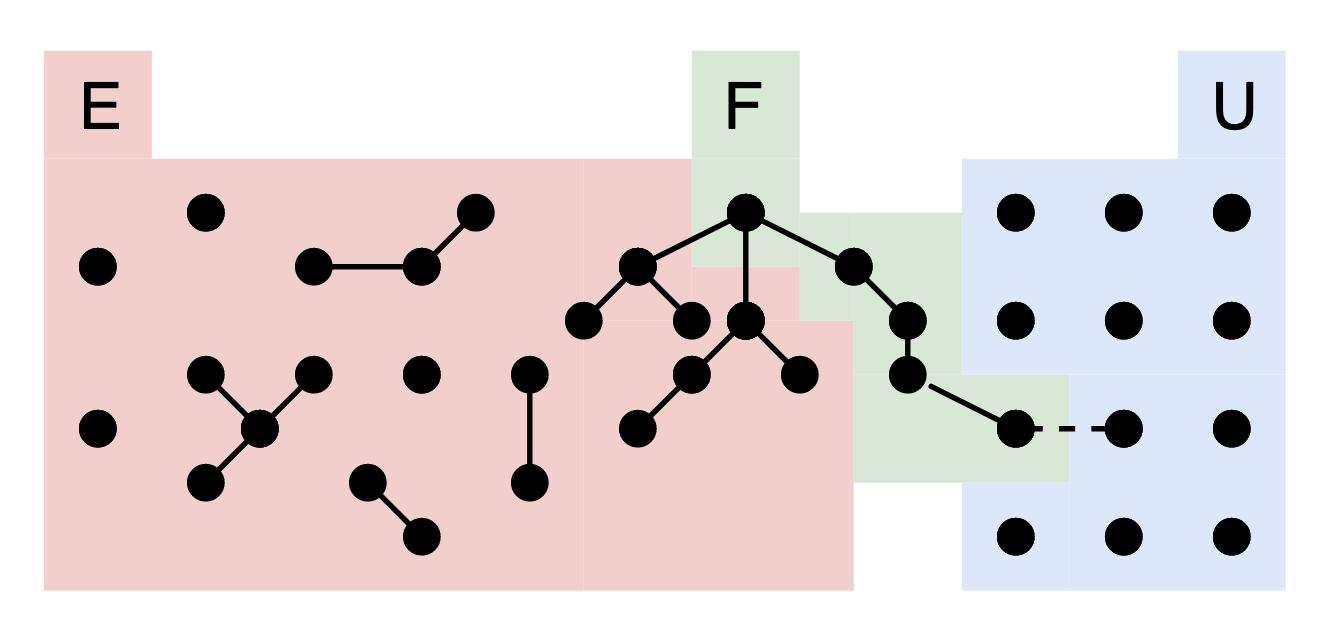
\includegraphics[width=0.75\textwidth]{aulas/10_17/dfs.png}
\end{figure}

\begin{observacao}
  Dado que o valor esperado de queries com resposta positiva é $\delta\,n^2\,p=\delta\left(1+\epsilon\vphantom{1j}\right)$, com probabilidade $\rightarrow1$, temos que o número de respostas positivas é
  \[
    \delta\left(1+\nicefrac{\epsilon}{2}\vphantom{1j}\right)n \leq s \leq \delta\left(1+2\,\epsilon\vphantom{1j}\right)n
  \]
  
  Pela inequação de Chebyshev ou pela de Chernoff.
  
  Sem perda de generalidade, assumiremos $\epsilon\leq\nicefrac{1}{4}$.
\end{observacao}

\begin{fato}
  $\not\exists$ arestas em $G\left(n,\ p\vphantom{1j}\right)$ entre $E$ e $U$, Pelo invariante da DFS.
\end{fato}

Provamos que, se $L_1\left(G\left(n,\ p\vphantom{1j}\right)\vphantom{1j}\right)<\nicefrac{1}{24}\,\epsilon^2\,n$, então $\left|E\vphantom{1j}\right|\,\left|U\vphantom{1j}\right|>t$ no modelo $G_t$.

Isso é uma contradição.

Vamos provar que, em algum momento, $\left|F\vphantom{1j}\right|\geq\nicefrac{1}{24}\,\epsilon^2\,n$, c.c. $\left|E\vphantom{1j}\right|\,\left|U\vphantom{1j}\right|>t$.
% #endregion

% \documentclass[a4paper,12pt]{article}

\usepackage[brazilian]{babel}
\usepackage[utf8]{inputenc}
\usepackage[T1]{fontenc}
\usepackage{amsmath}
\usepackage{amssymb}

\begin{document}

\section{Aula 21 de Outubro de 2019}
\label{2019_10_21}

Da aula passada temos que:

\[\frac{1}{H}\geq\epsilon>0 ,\ p=\frac{1+\epsilon}{n}\]

Então $\mathbb{P}(L_1(G(n,p))\geq (1/24)\epsilon^2 n)$ converge para 1 quando $n\rightarrow\infty$.\\

Executamos $t=sn^2$ passos da busca em profundidade, onde $\sigma=\epsilon/4$, e paramos.Examinamos a estrutura neste momento.\\

Vamos provar que quase certamente $|F|\geq n\epsilon^2/24$ sendo que $L_1(G_p) \geq n\epsilon^2/24$, quase certamente.\\
Podemos supor que o número de arestas descobertas até este momento é tal que, com alta probabilidade,
\[(*)\sigma(1+\frac{2\epsilon}{n})n\leq A\leq \sigma (1+2\epsilon)\]

De fato $\mathbb{E}(A)=tp=\sigma n (1+\epsilon)$ e $Ap_i(t,p)$ e * ocorre quase certamente. Suponha que * ocorre e $\epsilon \leq\ 1/4 $.

\begin{fato}
$ |E|<2sn $
\end{fato}
\begin{proof}
Suponha o contrário. Considere o momento em que $ |E|=2sn$. Temos o seguinte:
\[|F|\leq1+A\leq1+\sigma(1+2\epsilon)n<2\sigma n\]
Dessa forma temos que:
\[\sigma n^2 = t \geq |E||U|\geq2\sigma n(n-|E|-|F|) \geq 2\sigma n (n-2\sigma n - 2\sigma n ) = 2 \sigma n^2 (1-4\sigma)\]

O que é uma contradição.\\
\end{proof}

\begin{fato}
 $|F|\geq(1/6)\epsilon\sigma n = (1/24)\epsilon ^2 n$
\end{fato}
\begin{proof}
Suponha o contrário, ou seja, que $|F|<(1/6)\epsilon\sigma n$.
Temos que $|E|+|F|\geq A = \delta (1+\frac{\epsilon}{3})n$, portanto, usando o resultado acima:

\[|E|>\sigma(1+2/3\epsilon)n-(1/6)\epsilon\sigma n = \sigma(1+\epsilon/2)n\]

Temos assim que $\sigma(1+\epsilon/2)n<|E|<2\sigma n$.\\

Sabemos, porém, que:

\[|E||U|-|E|(n-|E|-|F|)\]
\[\geq\sigma(1+\epsilon/2)n(n-\sigma(+\epsilon/2)n-(1/6)\epsilon\sigma n)\]
\[=\sigma n^2 (1+\epsilon/2)(1-\sigma-2/3\epsilon\sigma)\]
\[\geq\sigma n^2(1+\epsilon/6-\epsilon^2/6)\]
\[>\sigma n^2\]

Como $|E||U|\leq\sigma n^2$, chegamos em uma contradição.
\end{proof}

\begin{teorema}
Suponha que $0<\epsilon\leq1/2$, $p=(1+\epsilon/n)$. Então $\lim_{n\to\infty} \mathbb{P}(L_2(G_p)>(200/\epsilon^3)\log n)=0$
\end{teorema}
\begin{proof}
Para a prova, usaremos exploração em duas rodadas. Seja $p_1 = (1+\epsilon/2)/n$ e $p_2$ tal que $(1-p)=(1-p_1)(1-p_2)$.\\

Então $G(n,p)=G(n,p_1)\cup G(n,p_2)$, independentes. Temos $p=p_1+p_2-p_1p_2\leq p_1+p_2$, o que implica que  $p_2\geq\epsilon/2n$.\\

Sabemos que quase certamente $L_1(G,n,p_1))\geq(1/24)(\epsilon^2/4)n = (1/96)\epsilon^2n$.\\

Seja $C$ uma componente de $G(n,p_1)$ com $|V(C)|=L_1(G(n,p_1))$. Adicione as arestas de $G(n,p_2)$ com ambas as pontas em $V(G(n,p_1))\backslash V(C)$ ou $G(n,p_1)$, criando um novo grafo.\\ 

Seja $C'$ uma componente contida em $V(G(n,p_1))\backslash V(C)$ neste novo grafo.
Suponha que $|C'|\geq (200/\epsilon^3)\log n$. Adicione agora as arestas de $G(n,p_2)$ entre $V(C')$ e $V(C)$. A probabilidade de nenhuma aresta aparecer entre $C'$ e $C$ é:\\
\[(1-p_2)^{|V(C)||V(C')|}\]
\[\leq e^{-p_2|V(C)||V(C')|}\]
\[\leq  e^{-\frac{\epsilon}{2n}}\frac{1}{96}\epsilon^2 n \frac{200}{\epsilon^3}\log n\]
\[=n^{-\frac{-2\epsilon}{27}}\rightarrow\]

Como o número de tais $C'$ é menor ou igual a n, temos pela cota da união que a probabilidade de que alguma delas não é "absorvida" por $C$ é menor ou igual a $n^{-\frac{1}{24}}$, o que tende a zero, como queríamos demonstrar.\\

\end{proof}

\end{document}

% \section{Aula 24 de Outubro de 2019}
\label{2019_10_24}

\subsection{Revisão de distribuição binomial}
$X\sim Bi(n,p)$
\\
(1) 
\[\mathbb{P}(X \geq k) \leq {n\choose k}p^{k} \leq {enp\choose k}^{k}\]
\\
(2)
\[\mu = \mathbb{e}(X) = np \]
(a)
\[\mathbb{P}(X \geq \mu +t) \leq exp(\frac{t^{2}}{-2(\mu+\frac{t}{3})})\]
(b)
\[\mathbb{P}(X \leq \mu -t) \leq exp(\frac{-t^{2}}{2\mu}) \leq exp(\frac{-\epsilon^{2}(k-1)^{2}}{2((k-1)(1-\epsilon)+\epsilon\frac{k-1}{3})}) \]
\[\leq exp(\frac{-\epsilon^{2}(k-1)^{2}}{2(k-1)}) \]
\\
(3)
\\
Se $ 0 \leq \epsilon \leq \frac{3}{2} $, então
\\
(a)
\\
\[\mathbb{P}(X \geq (1+\epsilon)\mu) \leq exp(\frac{-\epsilon^{2}\mu}{3}) \]
(b)
\[\mathbb{P}(X \leq (1-\epsilon)\mu) \leq exp(\frac{-1}{2}\epsilon^{2}\mu) \]
\\
\subsection{Grafos aleatórios (continuação)}
\begin{teorema}
$p = \frac{1 - \epsilon}{n} $, $\epsilon > 0$ constante.
\\
$L_{1}(G_{p}) \leq \frac{3}{\epsilon^{2}} log(n)$ quase certamente.
\end{teorema}
\\
\textbf{Prova:}\\

\[p = \frac{1-\epsilon}{n} < \frac{1-\epsilon}{n-1}\]
\\
Fixe $v\in V(G_{p})$\\

\begin{fato}
\[|V(C_{v})| \geq k \rightarrow \sum_{1\leq i \leq k} z_{i} \geq k-1\]
\end{fato}
\\
Assim,

\begin{align*}
	\mathbb{P}(|V(C_{v})|\geq k) \leq \mathbb{P}( \sum_{1\leq i \leq k} z_{i} \geq k-1) \\
	&\leq \mathbb{P}(\sum_{1\leq i \leq k} Bi(n-1,\frac{1-\epsilon}{n-1}) \geq k-1) \\
	&\leq e^{\frac{-1}{2}\epsilon^{2}(k-1)}
\end{align*}

Se \[k > (\frac{3}{\epsilon^{2}}log(n) \geq 1 + \frac{5}{2\epsilon^{2}} log(n) \] 
 
Então \[\mathbb{P}(|V(C_{v})| \geq k) \leq e^{\frac{-5}{4}log(n)} = \frac{1}{n^{\frac{5}{4}}}\]

Portanto,

\[\mathbb{P}(\exists v: |V(C_{v})|>k) \leq n \frac{1}{n^{\frac{5}{4}}} \rightarrow 0 \]

\begin{flushright}
$\square$
\end{flushright}\\

Para $v$ fixo, \[\mathbb{e}(|V(C_{v})|) \leq \frac{3}{\epsilon^{2}} \]

\begin{teorema}
Fixe $v\in V(G_{p})$ e suponha $\epsilon \leq \frac{1}{2}$ \\
Então
\[\mathbb{e}(|V(C_{v})|) \leq \frac{3}{\epsilon^{2}} \]
\end{teorema}\\
\textbf{Prova:} \\
Vimos que $\mathbb{P}(|V(C_{v})|\geq k) \leq e^{\frac{-1}{2}\epsilon^{2}k}$
\\
Seja $X = |V(C_{v})|$
\\
Temos
\begin{align*}
	\mathbb{e}(X) = \sum_{k \geq 1} k\mathbb{P}(X=k) = \sum_{k \geq 1} \mathbb{P}(X \geq k) \\
	&\leq \sum_{k \geq 1} e^{\frac{-1}{2}\epsilon^2(k-1)} \\
	&\leq  1 + e^{\frac{-1}{2}\epsilon^2} + e^{\frac{-1}{2}\epsilon^2 2} + ... \\
	&= \frac{1}{1-e^{\frac{-\epsilon^{2}}{2}}} \\
	&\leq \frac{1}{1-(1-\frac{\epsilon^{2}}{3})} \\
	& = \frac{3}{\epsilon^2}
\end{align*}

\begin{flushright}
$\square$
\end{flushright}\\

\begin{teorema}
\[p = \frac{1-\epsilon}{n}, \epsilon > 0.\] Então, quase certamente, toda componente de $G_{p}$ é ou uma árvore ou tem um único circuito.
\end{teorema}

\begin{lema}
(Teorema de Cayley)\\
O número de árvores rotuladas com $k$ vértices é $k^{k-2}$
\end{lema}\\

\textbf{Prova do teorema:}\\

Seja $X_{k}$ o número de componentes de $G_{p}$ com $k$ vértices e $\geq k+1$ arestas.\\
Queremos provar que \[\mathbb{P}(\sum_{k\geq 1} X_{k}>0) \rightarrow 0\].\\
Pelo teorema \[L_{1}(G_{p}) \leq C_{\epsilon}log(n)\]\\
Basta estimar \[\mathbb{P}(\sum_{1\leq k \leq(\frac{3}{\epsilon^2})log(n)} X_{k} > 0)\]\\
Temos que, para \[k \leq(\frac{3}{\epsilon^2})log(n)\]
\[\mathbb{e}(X_{k})\leq {n\choose k}k^{k-2}({{k\choose 2}\choose 2})p^{k-1} (1-p)^{k(n-k)}\]
\begin{align*}
	  \leq  (\frac{en}{k}kp(1-p)^{n-k})^{k}\frac{1}{k^{2}}\frac{k^{4}}{8}p \\
	  &\leq (e(1-\epsilon e^{-p(n-k)}))^{k}\frac{k^2}{8}\frac{1-\epsilon}{n} \\
	  &\leq ((1-\epsilon)e^{\epsilon})^{k}e^{pk^{2}}\frac{k^2}{8n} \\
	  &\leq \frac{k^{2}}{4n}(e^{\epsilon+log(1-\epsilon)})^{k} \\
	  &\leq \frac{k^{2}}{4n}(e^{\frac{-\epsilon^{2}}{2}})^{k}
\end{align*}
Concluímos que
\begin{align*}
	\mathbb{P}(\sum_{1\leq k \leq \frac{3}{\epsilon^{2}}log(n)}X_{k}\geq 1) \leq \mathbb{e}(\sum_{1\leq k \leq \frac{3}{\epsilon^{2}}log n}X_{k}) \\
	&= \sum_{1\leq k \leq \frac{3}{\epsilon^{2}}log(n)} \mathbb{e}(X_{k}) \\
	&\leq \sum_{1\leq k \leq \frac{3}{\epsilon^{2}}log(n)}\frac{k^{2}}{4n} e^{\frac{-\epsilon^{2}k}{2}} \\
	&\leq (\frac{3}{\epsilon^{2}}log(n))^{2}\frac{1}{4n}\sum_{k \geq 1} e^{\frac{-\epsilon^2 k}{2}} \leq \frac{3}{\epsilon^{2}} \\
	&\leq \frac{3^{3}}{4\epsilon^{6}}\frac{(log(n))^{2}}{n} \rightarrow 0
\end{align*}

\begin{flushright}
$\square$
\end{flushright}\\

\subsection{Cuckoo Hashing}\\

Colisões: maior lista ou cluster determina o pior caso. Qual o tamanho dela?
\\
Para n bolas e n urnas, qual o número de bolas nas urnas mais cheias?
\\
$X_{i}$ = número de bolas na urna i
\[X_{i}\sim Bi(n,\frac{1}{n})\]
\[\mathbb{P}(X_{i}\geq k) \leq {enp\choose k}^{k} = (\frac{e}{k})^{k}\]
$\mathbb{P}(\exists$ urna com $\geq k$ bolas) $\leq n\mathbb{P}(X_{i}\geq k) = n(\frac{e}{k})^{k}$
\\
Suponha $k = \frac{4(log(n))}{log(log(n))}$
\\
Então temos
\begin{align*}
	log(n)+ k(1-log(k)) \\
	&\leq log(n) + \frac{4log(n)}{log(log(n))}(1-(log(log(n)))+log(log(log(n)))) \\
	&\leq log(n) + \frac{4log(n)}{log(log(n))}(\frac{-1}{2}log(log(n))) \\
	&= -log(n)
\end{align*}
\\
Assim, $n{e\choose k}^{k}\leq\frac{1}{n}\rightarrow 0$\\

\begin{flushright}
$\square$
\end{flushright}\\

Portanto a maior lista é O($\frac{log(n)}{log(log(n))}$)\\

\textbf{Usando pares de urnas}\\
Para cada bola, sorteiam-se duas urnas e ela vai para a menos cheia
\\
Neste esquema, as urnas tem todas com probabilidade $1-o(1)$, no máximo
$\frac{1}{2}log(log(n)) + O(1)$ bolas
\\
\textbf{Cuckoo Hashing}\\
Pior caso de busca/remoção é O(1), e de inserção é O(1) amortizado.

\newpage
\part{BIBLIOGRAFIA}

%\bibliographystyle{amsplain}
\bibliography{bibliography}

\endgroup
\end{document}

%%% Local Variables:
%%% mode: latex
%%% eval: (auto-fill-mode t)
%%% eval: (LaTeX-math-mode t)
%%% eval: (flyspell-mode t)
%%% TeX-master: t
%%% End:
